\documentclass[12pt]{article}
\usepackage[utf8]{inputenc}
\usepackage[a4paper]{geometry}
%Y(6.5): JET (to the best of my knowledge) do not require margin of 1.25'', so I have reduced it to 1''
\geometry{verbose,tmargin=1in,bmargin=1in,lmargin=1in,rmargin=1in}
\usepackage{color}
\usepackage{array}
\usepackage{verbatim}
\usepackage{multirow}
\usepackage{amsmath}
\usepackage{amsthm}
\usepackage{graphicx}
\usepackage{setspace}
\usepackage[authoryear]{natbib}
\setstretch{1.5}
\usepackage[unicode=true,
 bookmarks=false,
 breaklinks=false,pdfborder={0 0 0},pdfborderstyle={},backref=false,colorlinks=true]
 {hyperref}
\hypersetup{
 citecolor=blue, linkcolor=blue, urlcolor=blue}

\makeatletter

%%%%%%%%%%%%%%%%%%%%%%%%%%%%%% LyX specific LaTeX commands.
%% Because html converters don't know tabularnewline
\providecommand{\tabularnewline}{\\}

%%%%%%%%%%%%%%%%%%%%%%%%%%%%%% Textclass specific LaTeX commands.
\numberwithin{equation}{section}
\numberwithin{figure}{section}
\theoremstyle{definition}
\newtheorem{defn}{\protect\definitionname}
\theoremstyle{plain}
\newtheorem{assumption}{Assumption}
\theoremstyle{plain}
\newtheorem{prop}{\protect\propositionname}
\theoremstyle{plain}
\newtheorem{thm}{\protect\theoremname}
\theoremstyle{remark}
\newtheorem{rem}{\protect\remarkname}
\theoremstyle{plain}
\newtheorem{lem}{\protect\lemmaname}
\theoremstyle{plain}
\newtheorem{cor}{\protect\corollaryname}
\newtheorem{fact}{Fact}
\newtheorem{factproof}{Proof of Fact}


%%%%%%%%%%%%%%%%%%%%%%%%%%%%%% User specified LaTeX commands.
%\usepackage{fullpage}
\usepackage[T1]{fontenc}
\usepackage{lmodern}
\definecolor{green}{RGB}{00, 180, 00}
\definecolor{red}{RGB}{180, 00, 00}
\usepackage{amsfonts}

\makeatother

\providecommand{\corollaryname}{Corollary}
\providecommand{\definitionname}{Definition}
\providecommand{\lemmaname}{Lemma}
\providecommand{\propositionname}{Proposition}
\providecommand{\remarkname}{Remark}
\providecommand{\theoremname}{Theorem}
\def\t{\theta}
\def\D{\Delta}
\def\e{\epsilon}

\begin{document}
\title{{\large{}Sampling Dynamics and Stable Mixing in Hawk--Dove Games\\}}
\author{Srinivas Arigapudi\thanks{
Department of Economics, Bar-Ilan University; Faculty of Industrial Engineering and Management, Technion. email: \protect\href{mailto:arigapudi@campus.technion.ac.il}{arigapudi@campus.technion.ac.il}.}
\and Yuval Heller\thanks{Department of Economics, Bar-Ilan University. email: \protect\href{mailto:yuval.heller@biu.ac.il}{yuval.heller@biu.ac.il}. }
\and Amnon Schreiber\thanks{Department of Economics, Bar-Ilan University. email: \protect\href{mailto:amnon.schreiber@biu.ac.il}{amnon.schreiber@biu.ac.il}. }
\thanks{We thank Daniel Friedman, Itay Kavaler, Ron Peretz, Ernst Schulte-Geers, Daniel Stephenson, Jiabin Wu, and seminar audiences at Bar-Ilan University and the University of Haifa for various helpful comments. We thank  Luis R. Izquierdo and Segismundo S. Izquierdo for their help in implementing the simulations using ABED software. YH and SA  gratefully acknowledge the financial support of the European Research
Council (\#677057) and the Israeli Science Foundation (\#2443/19). SA is supported in part at the Technion by a Fine Fellowship.
}}
%y: Amnon, If you want, you can thank your ISF grant.
\maketitle
\begin{abstract}
The hawk--dove game admits two 
types of equilibria: an asymmetric pure equilibrium in which players in one population play “hawk'' and players in the other population play ``dove,'' and an 
inefficient symmetric  mixed equilibrium, 
in which hawks are frequently matched against each other.
The existing  
literature shows that populations will converge to playing one of the 
pure equilibria  from almost any initial state. By contrast, we show that plausible sampling dynamics, in which agents occasionally revise their actions by observing either opponents' behavior or payoffs in a few past interactions, can induce the opposite result:  global convergence to one of the inefficient mixed stationary states.

\textbf{Keywords: }Chicken game, learning, evolutionary stability, bounded rationality, payoff sampling dynamics, action sampling dynamics.\\
\textbf{JEL codes: }C72, C73.
\end{abstract}

\section{Introduction}

The hawk--dove game is 
widely used to study situations of conflict between strategic participants. As a simple motivating example,
consider a situation in which a buyer (Player 1) and a seller (Player 2) have to bargain over the price of an asset (e.g., a house). Each player has two possible bargaining strategies (actions): insisting on a more favorable price (referred to as being a ``hawk''), or agreeing to a less favorable price in order to close the deal (being a ``dove''). The payoffs of the game are presented in Table \ref{tab:canonical-Hawk--dove-Games-1}. 
Two doves agree on a price that is equally favorable to both sides, and obtain a relatively high payoff, which is normalized to 1. A hawk obtains a favorable price when being matched with a dove, which yields her an additional gain of $g\in(0,1)$, at the expense of her dovish opponent.\footnote{
Our formal model studies a broader class of generalized hawk--dove games, in which the gain of a hawkish player might differ from the loss of the dovish opponent (as shown in Table \ref{tab:Generalized-Hawk--dove-Games} in Section \ref{sec:model}).} 
 Finally, two hawks obtain the lowest payoff of 0, due to a substantial probability of bargaining failure.
\footnote{
Our one-parameter payoff matrix is equivalent to the commonly used two-parameter payoff matrix (\citealp{smith1982evolution}), in which a dove obtains $\frac{V}{2}$ against another dove and 0 against a hawk, and a hawk obtains $\frac{V-C}{2}$ against another hawk and $V$ against a dove. Specifically, our one-parameter matrix is obtained from the two-parameter matrix by the affine transformation of adding the constant $\frac{C-V}{2}$ and dividing all payoffs by $\frac{C}{2},$ followed by substituting $g\equiv\frac{V}{C}.$}

 Observe that large values of $g$ (close to 1) correspond to environments that are advantageous to hawks (i.e., being a hawk yields a higher expected payoff against an opponent who might play either action with equal probability), small values of $g$ correspond to environments that are advantageous to doves, and values of $g$ that are close to 0.5 correspond to approximately balanced environments.

\begin{table}
\begin{centering}
\caption{Payoff Matrix of the Standard Hawk--Dove Game ($g\in\left(0,1\right)$) \label{tab:canonical-Hawk--dove-Games-1}}
\par\end{centering}
\smallskip{}
\centering
    \setlength{\extrarowheight}{2pt}
    \begin{tabular}{cc|c|c|}
      & \multicolumn{1}{c}{} & \multicolumn{2}{c}{\textcolor{red}{Player 2}}\\
      & \multicolumn{1}{c}{} & \multicolumn{1}{c}{$\textcolor{red}{h}$}  & \multicolumn{1}{c}{$\textcolor{red}{d}$} \\\cline{3-4}
      \multirow{2}*{\textcolor{blue}{Player 1}}  & $\textcolor{blue}{h}$ & $\textcolor{blue}{0},\textcolor{red}{0}$ & $\textcolor{blue}{1+g},\textcolor{red}{1-g}$ \\\cline{3-4}
      & $\textcolor{blue}{d}$ & $\textcolor{blue}{1-g},\textcolor{red}{1+g}$ & $\textcolor{blue}{1},\textcolor{red}{1}$ \\\cline{3-4}
    \end{tabular}
  \end{table}


The hawk--dove game 
(also known as the chicken game; see, e.g., \citealp{rapoport1966game,aumann1987correlated}) has been employed in modeling various strategic situations, such as: provision of public goods (\citealp{lipnowski1983voluntary}), nuclear deterrence between superpowers (\citealp{brams1987threat};  \citealp{dixit2019we}), industrial disputes (\citealp{bornstein1997cooperation}), bargaining problems (\citealp{brams2001fallback}), conflicts between countries over contested territories (\citealp{baliga2012strategy,baliga2020strategy}), and task allocation among members of a team (\citealp{herold2020evolution}). 

The hawk–dove game admits three Nash equilibria: two asymmetric pure equilibria, and 
an inefficient symmetric mixed equilibrium. In the pure equilibria (in which one of the players plays hawk while the opponent plays dove), all conflicts are avoided at the cost of inequality, as the payoff of the hawkish player is substantially higher than that of the dovish opponent. By contrast, in the symmetric mixed equilibrium 
both players obtain the same expected payoff,
yet this payoff is relatively low due to the positive probability of a conflict arising between two hawks. 

A natural question is to ask which equilibrium is more likely to obtain. Standard game theory is not helpful in answering this question, as all these Nash equilibria satisfy all the standard refinements (e.g., perfection). By contrast, the dynamic (evolutionary) approach can yield sharp predictions (for textbook expositions, see \citealp{weibull1997evolutionary,sandholm2010population}).

\paragraph{Revision dynamics}

Consider a setup in which pairs of agents from two infinite populations are repeatedly matched at random times (each such match of an agent from population 1 is against a new opponent from population 2).\footnote{Our paper focuses on two-population dynamics in which players condition their play on their role in the game. By contrast, in a one-population model, players cannot condition their play on their role in the game. The predictions of the one-population model are briefly discussed in Remark \ref{rem-two-one}.} Agents occasionally die (or, alternatively, agents occasionally receive opportunities to revise their actions). New agents observe some information about the aggregate behavior and the payoffs, and use this information to choose the action they will play in all future encounters. We are interested in characterizing the stable rest points of such revision dynamics, which can be used as an equilibrium refinement.

%S(12.5): The sentence which describes monotonicity, "the frequency of the strategy that yields the higher payoff (among the two feasible strategies) increases" can perhaps be rephrased by replacing the word frequency with growth rates?
%Y(12.5): If we replace "Frequency" with growth rate, we will have a longer and somewhat more cumbersome phrasing: the growth rate of the stratergy that yields the higher payoff is positive. Why do your prefer to use "growth rate"? how would you phrase it with growth rate?
%S(12.5): Since monotonicity is normally stated in terms of growth rate, I had a slight prefernce to state it that way. But with only two strategies, since growth rates and frequencies are equivalent, the current version is also good.
Most existing models assume that the revision dynamics are \emph{monotone} (also known as sign-preserving) with respect to the payoffs: the frequency of the strategy that yields the higher payoff (among the two feasible strategies) increases. A key result in evolutionary game theory is that in a hawk--dove game, all monotone
(two-population) revision dynamics converge to the asymmetric pure equilibria  from almost any initial state (henceforth, \emph{global convergence}; see \citealp{smith1976logic}, for the classic analysis, \citealp{smith1982evolution}, for the textbook presentation, \citealp{sugden1989spontaneous}, for the economic implications, and \citealp{oprea2011separating}, for the general dynamic result.)  Thus, the existing literature predicts that an efficient convention 
will emerge in which trade always occurs and most of the surplus goes to one side of the market. Casual observation suggests that this prediction might not fit well the behavior in situations such as the motivating example, in which the surplus of trade is typically divided relatively equally between the two sides of the market, and in which bargaining frequently fails.

In many applications, precise information about the aggregate behavior in the population  may be difficult or costly to obtain. In such situations, new agents have to infer the aggregate behavior in the population from a small sample of other players. 
In what follows, we 
study two plausible inference procedures, both of which violate monotonicity. The first procedure is the \emph{action-sampling dynamics} (also known as sampling best-response dynamics;  \citealp{sandholm2001almost,osborne2003sampling}). In these dynamics, each new agent observes the behavior of $k$ random opponents, and then adopts the action that is a best reply to her sample (with an arbitrary tie-breaking rule). 

In some applications, new agents may not be able to observe  opponents' actions, or they may lack information about the payoff matrix. Plausible revision dynamics in such situations are the \emph{payoff-sampling dynamics}  (also known as best experienced payoff dynamics; \citealp{osborne1998games,sethi2000stability}). 
In these dynamics, each new agent observes the payoffs obtained by incumbents of her own population in $k$ interactions in which these incumbents played hawk, and in $k$ interactions in which these incumbents played dove. Following these observations, the new agent adopts the action that yielded the higher mean payoff.
%Y(22.5): Removed for brevity "(with an arbitrary tie-breaking rule)."

We analyze both sampling dynamics in the hawk--dove game. In our analysis, we allow agents to have heterogeneous sample sizes (i.e., each new agent is endowed with a sample size of $k$ that is randomly chosen from an exogenous distribution). 
It is relatively straightforward to show that these dynamics admit at least three stationary states: 
two asymmetric pure states, and an inefficient symmetric state.\footnote{
Although the  symmetric stationary state does not coincide with the symmetric Nash equilibrium, they share similar qualitative properties: namely, symmetry between the two populations, and inefficiency induced by frequent matching of two hawks.}$^{,}$
\footnote{In some cases, the dynamics admit also asymmetric mixed states,
as is demonstrated in Section \ref{sec:Numeric-Analysis}.} 

\paragraph{Global convergence to mixed states} 
We show that sampling dynamics can yield qualitatively different results compared to monotone dynamics in the hawk--dove game. Specifically, our first main result (Theorem \ref{thm:global-mixed} and Corollary \ref{cor:g=l}) presents a simple 
%Y(12.5): removed ``iff''
%S(12.5): I see both "iff" and "if". It should perhaps be just "if". May be we can skip footnote 6 ?
%Y(12.5): I kept the "iff" (and removed the "if"). I think it is good to use iff, specially because we write before "Roughly speaking".
%Y(12.5): OK - I tentaitvely removed the footnote below.
 condition for sampling dynamics to induce the opposite result (relative to monotone dynamics), namely, convergence to one of the mixed stationary states from any interior state. Roughly speaking, this happens iff the following three conditions hold:
 %\footnote{The quantitative versions of these three conditions are stricter for action-sampling dynamics, and less strict for payoff-sampling dynamics.} 
 (1) sufficiently many agents have small sample sizes, (2) 
the population includes some agents with relatively large sample sizes (though still below a threshold that is increasing in $|g-0.5|$), and (3) $g$  is not too close to 0.5. 

The key to our first main result is to characterize when populations that start near one of the pure equilibria get away from this equilibrium (allowing for convergence to a mixed stationary state).
Assume that initially almost all ($1-\e$) buyers are hawks, and almost all ($1-\e$) sellers are doves. Consider a new agent who bases her decision  on a sample of $k$ actions. The sample will have a single occurrence of the rare action with a probability of about $k\cdot \epsilon$ (while the probability of having two or more occurrences of the rare action is negligible). The presence of agents with small samples (Condition (1)) is necessary for moving away from the pure equilibrium, because for dove-favorable games (i.e., $g<0.5$), a single occurrence of a rare action can induce a new seller to be a hawk only if her sample is small 
(similarly, the presence of agents with small samples is necessary for inducing a new buyer to be a dove in hawk-favorable games, i.e., $g>0.5$).

In dove-favorable games, a single occurrence of a rare action can induce a new buyer to be a dove  even for 
%Y(6.5): added "relatively"
relatively large sample sizes up to a threshold, 
%Y(6.5): I added the end of sentence till brackets due to Remark 1 of referee 1.
where this threshold is larger the farther $g$ is from 0.5 
(and the same holds for inducing new sellers to be hawks in hawk-favorable games). Having a larger sample size $k$ %Y(5.6): I added the follwoing brackets (agian due to remark 1 of reivewer 1)
(up to the above-mentioned threshold) helps to increase the frequency of occurrence of rare actions,  which explains why having a sufficiently large expected sample size (Condition (2)) is necessary for moving away from the pure equilibrium. Finally, when the game is balanced between the two actions (i.e., $g$ is close to 0.5), a single occurrence of a rare action can change the behavior of a new agent (in both populations) only if her sample is relatively small, but in this case, the total frequency in which rare actions occur in the samples might be too small. This is why having a less balanced game 
(i.e., Condition (3) of $g$ not being too close to 0.5) induces the population to move away from a pure equilibrium.

\paragraph{Global Convergence to Pure States} 
Our next result focuses on the action-sampling dynamics. We show that the behavior of the population is qualitatevely different for homogeneous populations (in which all agents have the same sample size) and heterogeneous populations. Specifically, we show (Theorem \ref{thm:unstableinterior_ASD}) that all homogenous populations (with a sample size of at-least 2) converge from almost all initial states to one of the pure states under the action-sampling dynamics. By contrast, heterogeneous populations might converge from most initial states to a symmetric mixed state, even in setups in which most agents have relatively large sample sizes, and the pure states are asymptotically stable.

\paragraph{Symmetric mixed states}
In some cases, a mixed stationary state might be close to a pure stationary state: e.g., having few hawkish buyers and few dovish sellers. Our final results present sufficient  conditions under which the populations converge (at least from nearby initial states) to a symmetric mixed state, which is far from the pure equilibria in the sense of being  (1) \emph{egalitarian} (i.e., both populations have the same expected payoff), and (2) \emph{inefficient} (i.e., the frequency of two hawks being matched together is substantial.)

Theorem \ref{thm:stableinterior_PSD} shows that (local) convergence to an inefficient symmetric state holds for many distributions of sample sizes, as long as the samples are not too large
%Y(22.5): New end of sentence
and the hawkish gain $g$ is sufficiently large. Theorem \ref{thm:stableinterior_ASD} shows that (local) convergence to an inefficient symmetric state occurs also under the action-sampling dynamics, albeit for a relatively narrow (yet, relevant) domain of distributions of sample sizes in which most agents sample a single action, while a large share  of the remaining agents have relatively large sample sizes. 
The proofs of these results include 
%Y(22.5): removed \emph around "new techniques" for modesty
new techniques, which apply various properties of binomial distributions, and might be of independent interest.

Taken together, our results show that when agents have limited information about the aggregate behavior of the population (which seems plausible in various real-life applications, such as the motivating example of buyers and sellers of houses), then an egalitarian, yet inefficient, convention may arise in which bargaining frequently fails. 

\paragraph{Structure} 
Section \ref{related-literature} presents the related literature. Our model is described in Section \ref{sec:model}. Section \ref{sec:local stability pure states} presents a ``complete'' characterization for global convergence to one of the mixed stationary states. Section \ref{sec:local stability mixed states} presents various necessary and sufficient conditions for the  stability of the inefficient symmetric stationary state.
The analytic results of the paper are supplemented by a numeric analysis in Section \ref{sec:Numeric-Analysis}.
We conclude in Section \ref{sec:conclusion}. Formal proofs are presented in the appendices.

\section{Related Literature}\label{related-literature}
\paragraph{Related theoretical literature}

The action-sampling dynamics were pioneered by 
  \cite{sandholm2001almost} and \cite{osborne2003sampling}. \cite{oyama2015sampling} applied these dynamics to prove global convergence results in supermodular games. Recently, \cite{heller2018social} studied the conditions on the expected sample size 
    that implies global convergence for all payoff functions and all sampling dynamics.\footnote{   \cite{hauert2018effects} use the term ``sampling dynamics'' to refer to a variant  of the replicator dynamics, in which when an agent samples another agent and mimics the other agent's behavior, it is more likely that these two agents will be matched with each other. This is less related to our use of the notion of ``Sampling dynamics'', which is in line with the literature cited in the main text.}

  
  \cite{salant2020statistical} (see also \citealp{sawa2021statistical}) generalized the action-sampling dynamics by allowing new agents to use various procedures to infer from their samples the aggregate behavior of the opponents.  \citeauthor{salant2020statistical} pay special attention to \emph{unbiased} inference procedures in which the agent's expected belief about the share of opponents who play hawk coincides with the sample mean. Examples of unbiased procedures are maximum likelihood estimation, beta estimation with a prior representing complete ignorance, and a truncated normal posterior around the sample mean. In our setup, the payoffs are linear in the share of agents who play hawk, which implies that the agent's perceived best reply depends only on the expectation of her posterior belief. This implies that our results hold for any unbiased inference procedure.
  
  The present paper, similar to the papers cited above, studies deterministic dynamics in infinite populations. When there is convergence to a stable stationary state in such dynamics, the convergence is fast
  (\citealp{oyama2015sampling}).
  By contrast, stochastic evolutionary models (see, e.g., the seminal contribution of \citealp{young1993evolution}, 
  and the recent hawk--dove application in \citealp{Bilancini-et-al-2021}), which are also based on revising agents observing a finite sample of opponents' actions,  focus on the very long-run behavior of stochastic processes when players’ choice rules include the possibility of rare “mistakes” 
  (sufficient conditions for stochastic evolutionary models to yield fast convergence are studied in \citealp{kreindler2013fast,arieli2020speed}).
 
The payoff-sampling dynamics were pioneered by \cite{osborne1998games} and \cite{sethi2000stability} and later generalized in various respects by \cite{sandholm2020stability}. It has been used in a variety of applications, including price competition with boundedly rational consumers (\citealp{spiegler2006competition}), common-pool resources (\citealp{cardenas2015stable}), contributions to public goods (\citealp{mantilla2018efficiency}), centipede games (\citealp{sandholm2019best}), finitely repeated games (\citealp{Raj}) and the prisoner's dilemma (\citealp{arigapudi2020instability}).
The existing literature assumes that all agents have the same sample size. 

A methodological contribution of the present paper is in extending the setup of payoff-sampling dynamics to analyze heterogeneous populations in which new agents differ in their sample sizes, and this heterogeneity leads to 
qualitatively new 
results.

It is well known that mixed stationary states in  multiple-population games cannot be asymptotically stable under the commonly used replicator dynamics (see, e.g.,  \citealp[Theorem 9.1.6]{sandholm2010population}).
 By contrast, we show that both classes of sampling dynamics, which are plausible in various real-life applications, can induce asymptotically stable mixed stationary states in a two-population hawk--dove game.

\paragraph{Related experimental literature}
\cite{selten2008stationary} experimentally tested the predictive power of various solution concepts in two-action, two-player games with a unique completely mixed Nash equilibrium. They show that 
%Y(6.5): removed extra both
both the payoff-sampling equilibrium and the action-sampling equilibrium outperform the predictions of both the Nash equilibrium and the quantal-response equilibrium. 


Recently, \cite{stephenson2019coordination} tested the predictive validity of various evolutionary models in coordinated attacker–defender games.\footnote{Experiments that directly test the dynamic predictions of evolutionary game theory are quite scarce. Two notable exceptions are the experiments showing the good fit of the dynamic predictions in the rock--paper--scissors game (\citealp{cason2014cycles,hoffman2015experimental}).} \citeauthor{stephenson2019coordination}'s experimental design is very favorable for monotone dynamics because each participant is shown the exact (population-dependent) payoff that would be obtained by each action at each point in time. Nevertheless, subjects frequently violate monotonicity: 10\%--20\% of the subjects switch from higher-performing strategies to lower-performing strategies.

The key prediction of monotone dynamics for hawk–dove games (in which agents from one population are randomly matched with agents from another population) is experimentally tested in \cite{oprea2011separating} and \cite{benndorf2016equilibrium}. Both experiments apply an interface that is favorable to monotonicity (i.e., each participant is shown the exact population-dependent payoff of each action). Both experiments show that the prediction of monotone dynamics holds in this setup, and that the populations converge to an asymmetric pure equilibrium in which one population (say, the buyers) plays hawk and the other population (say, the sellers) plays dove. 

Consider a revised experimental design, where an agent observes only the behavior of her own opponent, rather than the aggregate behavior of the opposing population. An interesting testable prediction of our model is that in this experimental design, the populations are likely to converge to the symmetric stationary state in the relevant parameter domain (in particular, when $g$ is not too far from 1; see Figure
\ref{fig:numeric_figure}).\footnote{\cite{benndorf2016equilibrium, benndorf2021games} 
studied a more general setup in which each participant in each round is randomly matched with an opponent from the other population with probability $\kappa \in (0,1)$, and is randomly matched with an opponent from her own population with the remaining probability $1-\kappa$. Our theoretical  predictions fit the setup of $\kappa$ close to one.}


\section{Model}\label{sec:model}

\subsection{The Hawk--Dove Game}
Let $G=\{A,u\}$ denote a symmetric two-player hawk--dove game, where: 
\begin{enumerate}
\item $A=\{h,d\}$
is the set of actions of each player, and 
\item $u:A^2\rightarrow\mathbb{R}$
is the payoff function of each player.
 \end{enumerate}
Let $i\in\left\{ 1,2\right\} $ be an index referring to one of the
players, and let $j=\left\{ 1,2\right\} \backslash\left\{ i\right\} $
be an index referring to the opponent. We interpret action $h$
as the hawkish (more aggressive) action and $d$ as the dovish
action. The payoff matrix $u(\cdot,\cdot)$ of a generalized hawk--dove game is given in Table \ref{tab:Generalized-Hawk--dove-Games}.
When both agents are dovish, they obtain a relatively high payoff, which is normalized to 1. When both agents are hawkish, they obtain their lowest feasible payoff, which is normalized to 0. 
Finally, when one of the players is hawkish and her opponent is dovish, the hawkish player \emph{gains}  $g\in(0,1)$ (relative to the payoff 1 obtained by two dovish players), while her dovish opponent \emph{loses}\footnote{\cite{herold2020evolution} allow a broader 
domain in which the assumption of $g,l\in(0,1)$ is replaced with the weaker assumption of
$g>0$, $l<1,$ and $l+g>0$. All of our results hold in this extended setup.
} $l\in(0,1)$. 
The game admits three Nash equilibria: two asymmetric pure Nash equilibria: $(h,d)$ and $(d,h),$ and a symmetric mixed Nash equilibrium in which each player plays $h$ with probability $\frac{g}{1+g-l}$,
and obtains a relatively low expected payoff of $\frac{(1+g)(1-l)}{1+g-l}<1$.

\begin{table}
\begin{centering}
\caption{Payoff Matrix of a Generalized Hawk--Dove Game $g,l\in\left(0,1\right)$ \label{tab:Generalized-Hawk--dove-Games}}
\par\end{centering}
\smallskip{}
\centering
    \setlength{\extrarowheight}{2pt}
    \begin{tabular}{cc|c|c|}
      & \multicolumn{1}{c}{} & \multicolumn{2}{c}{\textcolor{red}{Player 2} \vspace{-0.5em}}\\
      & \multicolumn{1}{c}{} & \multicolumn{1}{c}{$\textcolor{red}{h}$}  & \multicolumn{1}{c}{$\textcolor{red}{d}$} \\\cline{3-4}
      \multirow{2}*{\textcolor{blue}{Player 1}}  & $\textcolor{blue}{h}$ & $\textcolor{blue}{0},\textcolor{red}{0}$ & $\textcolor{blue}{1+g},\textcolor{red}{1-l}$ \\\cline{3-4}
      & $\textcolor{blue}{d}$ & $\textcolor{blue}{1-l},\textcolor{red}{1+g}$ & $\textcolor{blue}{1},\textcolor{red}{1}$ \\\cline{3-4}
    \end{tabular}
  \end{table}
An important special 
subclass  is
the \emph{standard} hawk--dove games, 
in which $g=l$ (see Table \ref{tab:canonical-Hawk--dove-Games-1}); i.e., the gain of the hawkish player is equal to the loss of her dovish opponent.
%Y(12.5): New subsection's title
\subsection{Evolutionary Process}

We assume that there are two unit-mass continuums of agents 
(e.g., buyers and sellers) and that
agents in population 1 are randomly matched with agents in population
2. Aggregate behavior in the populations
at time $t\in\mathbb{R}^{+}$ is described by a \emph{state}
$\mathbf{p}\left(t\right)=\left(p_{1}\left(t\right),p_{2}\left(t\right)\right)\in\left[0,1\right]^{2}$,
where $p_{i}\left(t\right)$ represents the share of agents playing
the hawkish action $h$ at time $t$ in population $i$. We extend
the payoff function $u$ to states (which have the same
representation as mixed strategy profiles) in the standard linear
way. Specifically, $u(p_i,p_j)$ denotes the average payoff of population $i$ (in which a share $p_i$ of the population plays $h$)   
when randomly matched against population $j$ (in which a share $p_j$  plays $h$).
With a slight abuse of notation, we use $d$ (resp., $h$)
to denote a degenerate population in which all of its agents play action $d$ (resp., $h$).
A state $\mathbf{p}=\left(p_{1},p_{2}\right)$ is \emph{symmetric} if $p_{1}=p_{2}$. 
%Y(12.5): New sentence
A state $\mathbf{p}=\left(p_{1},p_{2}\right)$ is \emph{interior} (or mixed) if $p_1,p_2\in(0,1).$ 

Agents occasionally die and are replaced by new agents (equivalently,
agents occasionally receive opportunities
to revise their actions).
Let $\delta>0$ denote the death rate
of agents in each population, which we assume to be independent of
the currently used actions. It turns out that $\delta$ does not have any effect on the dynamics,
except to multiply the speed of convergence by a constant. 
The evolutionary process is represented by a continuous function
$\textbf{w}:\left[0,1\right]^{2}\rightarrow\left[0,1\right]^{2}$, which describes
the frequency of new agents in each population who adopt action $h$ as a function of the current state. That is, $w_{i}\left(\mathbf{p}\right)$
describes the share of new agents of population $i$ who adopt action
$h$, given state $\mathbf{p}$. 
Thus, the instantaneous change in the share of agents of population $i$ that play hawk is given by 
$\dot{p}_{i}=\delta\cdot\left(w_{i}\left(\mathbf{p}\right)-p_{i}\right).\label{eq:general-dyanmics}$

\begin{rem}\label{rem-two-one}
Our \emph{two-population} dynamics fit situations in which each player can condition
her play on her role in the game (being Player 1 or Player 2). Common examples of such situations are (1) when sellers are matched with buyers, as in the motivating example, and (2) when each player observes if she has arrived slightly earlier or slightly later at a contested resource (\citealp{smith1982evolution}).
%Y(6.5): New sentence due to R3's mis-understanding.
Our dynamics induce the same results as one-population dynamics over a larger game with  $2\times2$ “role-dependent” actions: being a hawk in both roles, being a dove in both roles, being a hawk as player 1 and a dove as player 2 (i.e., the “bourgeois” strategy of \citealp{smith1982evolution}), and being a hawk as player 2 and a dove as player 1).

By contrast, in \emph{one-population} dynamics 
of the original two-action game, an agent cannot condition her play on her role. It is well known that all monotone one-population dynamics converge to the unique mixed Nash equilibrium in hawk--dove games 
(see, e.g., \citealp[Section 4.3.2]{weibull1997evolutionary}). It is relatively straightforward to establish that one-population sampling dynamics lead to qualitatively similar results (convergence is to a somewhat different interior state than in
the mixed Nash equilibrium, but the comparative statics with respect to the payoff parameters remain similar).
\end{rem}
\paragraph{Monotone Dynamics}
The most widely studied 
dynamics are those that are monotone with respect to the payoffs.
A dynamic is monotone if the share
of agents playing an action increases iff the action yields a higher
payoff than the alternative
action.\footnote{In games with more than two actions, there are various definitions that capture different aspects of monotonicity. All these definitions coincide for two-action games. In particular, Definition \ref{def-monotone} coincides in two-action games with \citeauthor{weibull1997evolutionary}'s (\citeyear[Section 5.5]{weibull1997evolutionary}) textbook definitions of payoff monotonicity, payoff positivity, sign preserving, and weak payoff positivity.}$^{,}$\footnote{The best-known example of payoff monotone dynamics is the standard
replicator dynamic (\citealp{taylor1979evolutionarily}), which is
given by
$\dot{p}_{i}=w_{i}\left(\textbf{p}\right)-p_{i}=p_{i}\left(u\left(h,p_{j}\right)-u\left(p_{i},p_{j}\right)\right).\label{eq:replicator-dynamics}$}
\begin{defn}\label{def-monotone}
The dynamic $\textbf{w}:\left[0,1\right]^{2}\rightarrow\left[0,1\right]^{2}$
is \emph{monotone} if for any player $i$, any interior $p_{i}\in\left(0,1\right)$,
and any $p_{j}\in\left[0,1\right]$: $\dot{p}_{i}>0\,\,\Leftrightarrow\,\,u\left(h,p_{j}\right)>u\left(d,p_{j}\right).$ 
\end{defn}

\cite{oprea2011separating} showed that under monotone dynamics, from almost any initial state, the populations converge to one of the two asymmetric pure equilibria in which one population always plays
$h$ and the other population always plays $d$ (generalizing the seminal analysis of \citealp{smith1976logic}). 
%Y(6.5): I removed "For completeness, we state and prove an equivalent result, using the notation of our model, in Appendix \ref{subsec:benchmark}."

\subsection{Sampling Dynamics}
In what follows, 
we study two plausible nonmonotone dynamics, in which new agents base their choice on inference from small samples. 

\paragraph{Distribution of sample sizes}

We allow heterogeneity in the sample sizes used by new agents. Let
$\theta\in\Delta\left(\mathbb{Z}_{+}\right)$ denote the distribution
of sample sizes of new agents. A share of $\theta\left(k\right)$
of the new agents have a sample of size $k$. Let
$\text{supp}\left(\theta\right)$ denote the support of $\theta$,  let 
$\max($supp$(\theta))$ 
denote the maximal 
sample size in the support of
$\theta$, and let $\max($supp($(\theta))=\infty$ if $\theta$'s
support is unbounded.
If there exists some $k,$ for which $\theta(k)=1,$ then we use
$k$ to denote the degenerate (homogeneous) distribution $\theta\equiv k$.

\begin{defn}
An \emph{environment} is a tuple $E=(g,l,\theta)$ where $g,l\in (0,1)$ describe the underlying hawk--dove game, and $\t\in\D\left(\mathbb{Z}_{+}\right)$ describes the distribution of sample sizes. 
\end{defn}


\paragraph{Action-sampling dynamics}
The action-sampling dynamics (\citealp{sandholm2001almost}) fit situations in which agents do not know the exact distribution of actions being played in the opponent's population, but know the payoffs of the underlying game. Agents estimate the unknown distribution of actions by sampling a few opponents' actions. Specifically, each new agent with sample size $k$ (henceforth, a $k$-agent) samples
$k$ randomly drawn agents from the opponent's population and then adopts the action that is the best reply  against the sample. 
%Y(12.5): I changed it to italics so it won't be too-easily missed.
\emph{To simplify notation, we assume that in case of a tie, the new agent plays action $d$}. Our results are
%Y(9.5): I slightly rephrased to qualitatvely the same, and not the same, as we don't assume genereceity
qualitatively the same for any tie-breaking rule.

Let ${X}_{k}\left(p_{j}\right)\sim Bin\left(k,p_{j}\right)$
denote a random variable with binomial distribution with parameters
$k$ (number of trials) and $p_{j}$ (probability of success in each
trial), which is interpreted as the number of $h$-s in the sample. 
Observe that the sum of payoffs of playing action $h$ against the sample is $(1+g)\cdot(k-X_k(p_j))$ and the sum of payoffs of playing action $d$ against the sample is
%Y(6.5): Correcrted 1-->K twice, as spotted by reivewer 2.
$(k-X_k(p_j))+X_k(p_j)\cdot(1-l)=k-lX_k(p_j)$. 

This implies that action $h$ is the unique best reply to a sample of size $k$ iff $(1+g)(k-X_k(p_j)>k-lX_k(p_j)\Leftrightarrow \frac{X_k(p_j)}{k}<\frac{g}{1+g-l}$. This, in turn, implies that the action-sampling dynamic in environment $(g,l,\t)$ is given by
\begin{equation}
w^{A}\left(p_{j}\right)\equiv w_{i}^{A}\left(\textbf{p}\right) = \sum_{k\in \text{supp}\left(\theta\right)}\theta(k)\cdot\Pr\left(\frac{X_{k}\left(p_{j}\right)}{k}<\frac{g}{1+g-l}\right).\label{eq:action-sampling0dyanmics}
\end{equation}

\paragraph{Payoff-sampling dynamics}
The payoff-sampling dynamics (\citealp{osborne1998games}) fit situations in which agents either do not know the payoff matrix or do not have feedback about the actions being played in the opponent's population. Specifically, a new $k$-agent observes for each of her feasible actions the mean payoff obtained by playing this action in $k$ interactions (with each play of each action being against a newly drawn opponent), and then chooses the action whose mean payoff was highest. One possible interpretation for these observations is that each new $k$-agent tests each of the available actions $k$ times, and then adopts for the rest of her life the action with the highest mean payoff during the testing phase. As above, we assume that a tie induces a new agent to play  action $d$ (and the results are qualitatively the same for any tie-breaking rule). 

We refer to the sample against which action $h$ (resp.,
$d$) is tested as the $h$-sample (resp., $d$-sample). Let $X_{k}\left(p_{j}\right),Y_{k}\left(p_{j}\right)\sim Bin\left(k,p_{j}\right)$
denote two iid random variables with a binomial distribution with parameters $k$ and $p_{j}$. Random variable $X_{k}$ (resp., $Y_{k}$) is interpreted as the number of times in which the opponents have played action $h$ in the $h$-sample (resp., $d$-sample). 
Observe that the sum of payoffs of playing action $h$ (resp., $d$) against its $h$-sample (resp., $d$-sample) is $(1+g)(k-X_k(p_j))$ 
%Y(.65): corrected 1--. dur to R2.
(resp., $k-l Y_k(p_j$)).
This implies that action $h$ has the highest mean payoff  iff
%Y(6.5): added missing closing bracket (R2)
$(1+g)(k-X_k(p_j))>k-lY_k(p_j)\Leftrightarrow (1+g)X_k(p_j)<gk+lY_k(p_j)$. Thus the payoff-sampling dynamic in environment $(g,l,\t)$ is given by
\begin{equation}
w^{P}\left(p_{j}\right)\equiv w_i^{P}\left(\textbf{p}\right) =\sum_{k\in \text{supp}\left(\theta\right)}\theta(k)\cdot\Pr((1+g)X_k(p_j)<gk+lY_k(p_j)).\label{eq:payoff-smapling-dynamics}    
\end{equation}
Henceforth, we omit the superscript $A$ / $P$ (i.e., we write $w(p_j)$) when referring to properties that hold for both classes of dynamics.



\section{Global Convergence to Mixed States}\label{sec:local stability pure states}
Recall that under monotone dynamics the population converges from almost any initial state to one of the pure equilibria.
In this section, we fully characterize the  conditions for which the opposite result holds under sampling dynamics; i.e., the populations converge from almost any initial state to one of the mixed (interior) stationary states.

\subsection{Analysis of $w(p_1)$ and Preliminary Results}
%Y(8.5): A new (or ehavily revised) subsection. A & S - Please read carefully and revise/comment.
The dynamic characteristics of both classes of sampling dynamics are closely related to the properties of the polynomial 
%Y(23.5): I cahnged w(p_j) to w(p_1) in the follwoing two paragraphs
$w(p_1)$, its inverse $w^{-1}(p_1)$ and their intersection points, which are analyzed in this subsection.

Figure \ref{figure-generic} illustrates the phase plots of the sampling dynamics and the properties of the polynomial $w(p_1)$ and its inverse $w^{-1}(p_1)$  for the environment in which $g=l=0.25$ and $\theta\equiv3$. The green solid curve is the polynomial $p_2=w(p_1)$, which describes the states in which $\dot p_1=0$. The orange dashed curve is the polynomial $p_2=w^{-1} (p_1).$ 

\begin{figure}
\begin{centering}
 \caption{Illustrative Phase Plots ($g=l=0.25$ and $\theta\equiv3$)  \label{figure1}}

 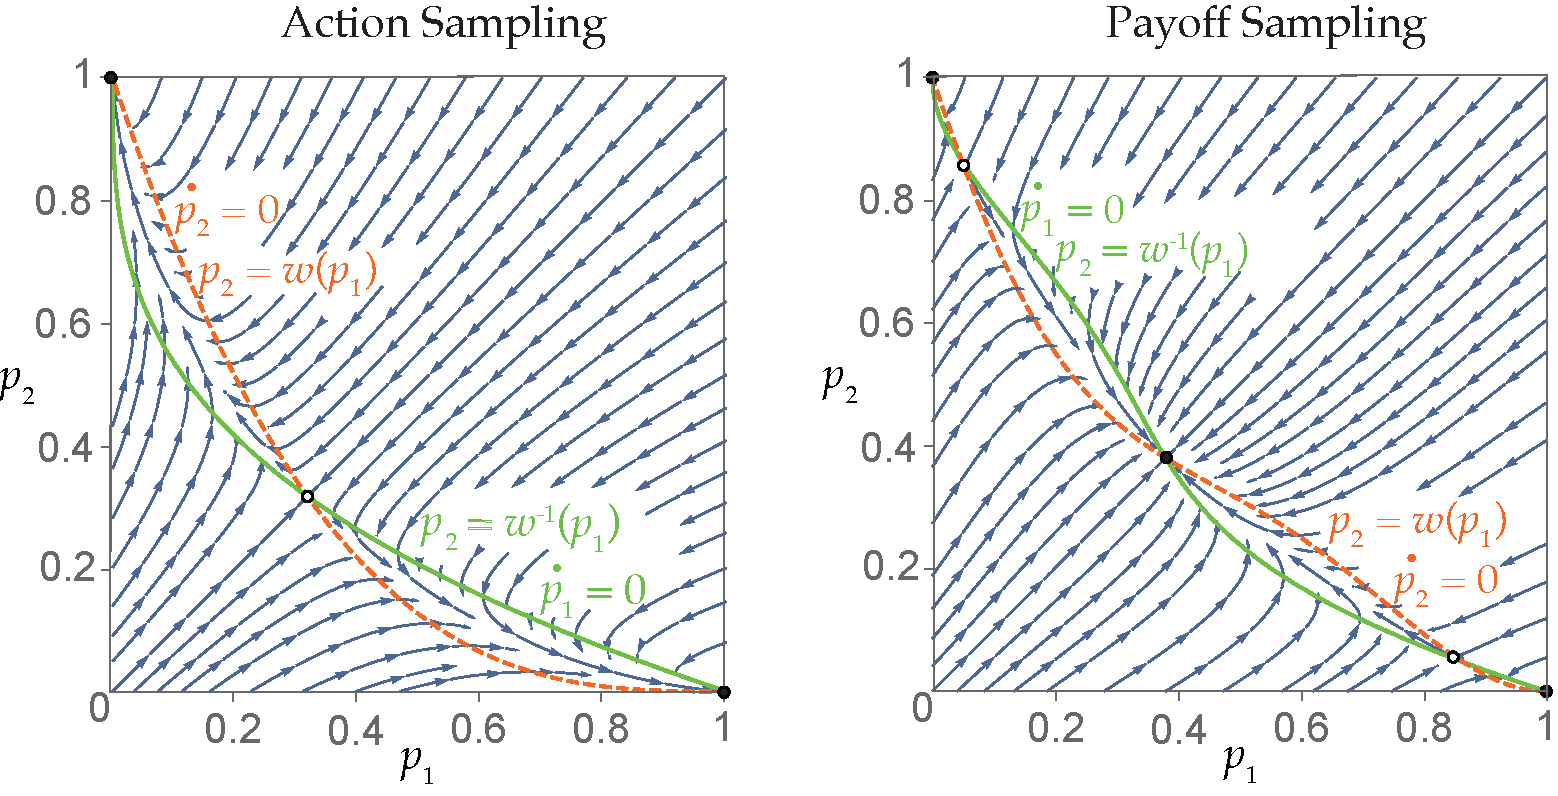
\includegraphics[scale=0.6]{Figures/generic-plots.pdf}\label{figure-generic}
\par\end{centering}
    {\small{}
   The figure illustrates the phase plots of the action-sampling dynamics (left panel) and the payoff-sampling dynamics (right panel) for the environment  in which $g=l=0.25$ and $\theta\equiv3$. The solid green (resp., dashed orange) curved line shows the states in which $\dot p_1=0$. The intersection points of these curved lines are the stationary states. A solid (resp., hollow) dot represents an asymptotically stable (resp.,  unstable) stationary state.}{\small\par}
\end{figure}

%Y(8.5): Srinivas and Amnon, please read carefully the fact. If its correctness is not immediatly clear please add an argument or a brief proof.
 The following fact is immediate (for both classes of sampling dynamics) from  the basic properties of  $X_k$ and $Y_k$ as binomial random variables.
\begin{fact}\label{fact-w}
$w(p_j)$ is a 
%Y(6.5: added strictly
strictly decreasing polynomial function that satisfies $w(0)=1$ and $w(1)=0$.
%Y(6.5): added sentence on w^-1
This implies that the inverse function $w^{-1}:[0,1]\rightarrow[0,1]$ exists, is continuously differentiable, and that $w^{-1}(0)=1$ and $w^{-1}(1)=0.$
\end{fact}
Fact \ref{fact-w} implies that the two curves intersect at $(0,1)$, $(1,0)$ and at a unique symmetric state $(p,p)$. The curves might admit additional intersection points.

Appendix \ref{sub-standard-definitions} presents the standard definitions of  stationary states, asymptotically stable states and unstable states. Observe that a state is stationary
%Y(12.5): New sentence in brackets
(i.e., it is a fixed point of the dynamics) iff it is an intersection point of the two curves $w$ and $w^{-1}$.
%Y(8.5): S and A, please confirm that the fact is immediate. If it might require a short argument/brief proof, please add it.
%S(12.5): I think it is immediate.

\begin{fact}\label{fact-intersection}
State $(p_1,p_2)$ is stationary iff $w(p_1)=w^{-1}(p_1)=p_2$.
\end{fact}

Our first result shows that the population converges to one of the stationary states from any initial state.\footnote{
%Y(12.5): New footnote.
One could also prove Proposition \ref{pro-convergence-to-stationary} by relying on Bendixson--Dulac Theorem (see, Theorem 9.A.6 of \citealp{sandholm2010population}). We present a direct proof as the arguments are helpful in the proof of Proposition \ref{pro-convergence-to-pure-iff-asymp}.)}
\begin{prop}\label{pro-convergence-to-stationary}
  $\lim_{t\rightarrow\infty}\mathbf{p}\left(t\right)$ exists for any $\textbf{p}(0),$ and it is a stationary state.
\end{prop}
\begin{proof}[Sketch of Proof]
%Y(12.5): I have shortened the sketch to one paragraph
Observe that in any trajectory that begins above (resp., below) both curves, the share of hawks in both population decreases (increases), which implies that the trajectory move downward and to the left (resp., upward and to the right) until it intersects with one of the curves. Thus, we can focus on trajectories that begin between the two curves. Assume WLOG that the initial state is below 
 $w(p_1)$ and above  $w^{-1}(p_1)$ (the argument in the opposite case is analogous). In any such state the share of hawks in population 1 (resp., 2) increases (resp., decreases). This implies that the trajectory moves upward and to the left until meeting one of the curves. This meeting point must be an intersection point of both curves, because if the meeting point were only with $w(p_1)$ (resp., $w^{-1}(p_1)$), the trajectory there should have been  horizontal to the left (vertical upward), which implies that the trajectory should come from the right side of the curve (from below the curve), leading to a contradiction.  See Appendix \ref{proof-convergence-to-stationary} for a formal proof.
\end{proof}
Our second result shows that if any initial state converges to one of the pure equilibria, then this equilibrium must be asymptotically stable (as defined in Appendix \ref{sub-standard-definitions}).
\begin{prop}\label{pro-convergence-to-pure-iff-asymp}
Assume that  $\textbf{p}(0)\neq (1,0)$ and $\lim_{t\rightarrow\infty}\mathbf{p}\left(t\right)=(1,0)$, then $(1,0)$ is asymptotically stable. The same result holds when replacing $(1,0)$ with $(0,1).$
\end{prop}
\begin{proof}[Sketch of Proof]
%Y(12.5): I slightly shortend the sketch of proof
Due to analogous arguments to the above sketch of proof we can assume WLOG that $\textbf{p}(0)$ is between the two curves, and that the trajectory moves upward and to the left (which is required for convergence to (1,0)) iff the curve $w(p_1)$ is above $w^{-1}(p_1)$, and the closest intersection point of the two curves to the left of  $\textbf{p}(0)$ is (1,0). These two conditions imply that any initial state sufficiently close to (1,0) converges to (1,0), which implies that (1,0) is asymptotically stable.
See Appendix \ref{proof-converge-pure-iss-asymp} for the formal proof.
\end{proof}

\subsection{Single Appearance of a Rare Action}
The following lemma characterizes when a single appearance of a rare action in a new agent's sample can change the agent's behavior (see the proof in Appendix \ref{lem-proof}; 
%Y(9.5): New sentence
we require strictly higher payoffs for action $h$ and weakly higher payoffs for action $d$ due to our tie-breaking rule in favor of action $d$).
%S(12.5): Perhaps, it will be better if I add in an assumption environment stating our tie-breaking rule of favoring "d" in case of a tie.
%Y(12.5): I changed the tie-breaking rule to italics (in top paragraph in page 12). I think that this is suffcient. USing the Asusmption envrinement might suggest that it is a crucial/important asusmption.
%S(12.5): Sounds good.

\begin{lem}
\label{lemma-sample} Consider a new agent in population $i$ with a sample size of $k$.
\begin{enumerate}
\item Action-sampling dynamics: (I) Action $h$ induces a 
%Y(9.5): added strictly
strictly higher payoff
against a sample with a single opponent's action $d$ iff
%Y(9.5): I removed the floor notation and the footnote. \footnote{$\lfloor x\rfloor$ is the largest integer less than or equal to $x.$}
$k<\frac{1+g-l}{1-l}$ 
and (II) Action $d$ induces a
%Y(9.5): added weakly
weakly higher payoff against a sample
with a single $h$ iff $k\leq \frac{1+g-l}{g}$. 
\item Payoff-sampling dynamics: (I) a $h$-sample with a single action $d$
induces a
%Y(9.5): added strictly
strictly higher mean payoff than a $d$-sample with no $d$-s
iff $k<\frac{1+g}{1-l}$ and (II) a $d$-sample with no $h$-s
induces a weakly higher mean payoff than an $h$-sample with a single
$h$ iff $k\leq \frac{1+g}{g}$. 
\end{enumerate}
\end{lem}

Lemma \ref{lemma-sample} allows us to define the maximal sample sizes in which a single appearance of a rare action can change the behavior of a new agent.

%Y(9.5): Removed all "floor"s as it is problematic without genericity

\begin{defn}\label{def:maximal-samples}
Let 
 $\,m_{h}^{A}= 1+\frac{g}{1-l} ,\,m_{d}^{A}= 1+\frac{1-l}{g},
 m_{h}^{P}= \frac{1+g}{1-l} ,\,m_{d}^{P}= \frac{1+g}{g}.$
 
\end{defn}
%S(12.5): I think "A,P" can be written in normal font, like $A,P$ and not as $^{A,P}$.
%Y(12.5): OK. I did so.
    We omit the superscript ${A,P}$ when stating a result that is true for both dynamics; for example, we write $m_h$, which denotes $m_h^P$ when the underlying dynamics is payoff sampling, and which denotes $m_h^A$ when the underlying dynamics is action sampling. 
    
    The parameter $m_{h}$ is the maximal sample size for which
a single appearance of $d$ in the sample, when all other sampled actions are $h$, can induce a new agent to adopt action $h$. Similarly,  $m_{d}$ is the maximal sample size for which a single appearance of $h$ in the sample, when all other sampled actions are $d$, can induce a new agent to adopt action $d$. 
 
We conclude this subsection by presenting a definition of $m$\emph{-bounded expectation} of a probability distribution with support on the set of positive integers. It is the expected value of
the probability distribution by restricting its support to $m.$ Formally, we have:

\begin{defn}
The $m$\emph{-bounded expectation} $\mathbb{E}_{\leq m}$ (resp., $\mathbb{E}_{< m}$) of distribution $\theta$ with support on
%Y(12.5): removed for brevity "posiitve"
integers is:\footnote{
%Y(12.5): New footnote
Observe that in our notation the parameter $k$ takes only (positive) integer values (although we allow the upper bound $m$ to be non-integer).}
$\mathbb{E}_{\leq m}\left(\theta\right)=\sum_{1 \leq k\leq m}\theta\left(k\right)\cdot k$ (resp., $\mathbb{E}_{< m}\left(\theta\right)=\sum_{1\leq k< m}\theta\left(k\right)\cdot k$).
\end{defn}
\subsection{Asymptotic Stability of Pure Equilbria}
Our next result characterizes the asymptotic stability of the pure
states. It shows that the asymptotic stability depends only on whether the product of the bounded expectations of the distribution of sample sizes is larger or smaller than one, where the bound of each distribution is the maximal sample size for which a single appearance of a rare action can change the behavior of a new agent. Formally 
%Y(9.5): New sentence in brackets.
(where replacing the tie-breaking rule with a $h$-favorable one would replace the ``<''-s and the ``$\leq$''-s in the statement):
%Y(12.5): chnaged iff to if 
\begin{prop}
\label{prop:pure-equilbiria-satbility}
\begin{enumerate}
\item $\mathbb{E}_{< m_{h}}\left(\theta\right)\cdot \mathbb{E}_{\leq m_{d}}\left(\theta\right)>1\,\Rightarrow\,$ both pure stationary states are unstable.
\item $\mathbb{E}_{<m_{h}}\left(\theta\right)\cdot \mathbb{E}_{\leq m_{d}}\left(\theta\right)<1\,\Rightarrow\,$ both pure stationary states are asymptotically stable. 
\end{enumerate}
\end{prop}

\begin{proof}[Sketch of Proof]
Consider a slightly perturbed state $(\epsilon,1-\epsilon)$ near the pure equilibrium $(0,1).$ Observe that almost all agents in population 1 (resp.,  2) play $d$ (resp., $h$). 
The event of two rare actions appearing in a sample of a new agent has a negligible probability of $O(\epsilon^2)$. If a new agent has a sample size of $k$, then the probability of a rare action appearing in the sample is approximately $k \cdot \epsilon.$ This rare appearance changes the perceived best reply of a new agent of population 1 iff $k$ is smaller than $m_{h}$. Thus, the total probability that a new agent of population 1 (resp., 2) adopts a rare action 
is equal to $\mathbb{E}_{<m_{h}}\left(\theta\right)$ (resp., $\mathbb{E}_{\leq m_{d}}\left(\theta\right)$). This implies that the product of the share of new agents adopting a rare action in each population is $\epsilon\cdot\mathbb{E}_{< m_{h}}\left(\theta\right)\cdot\e\cdot\mathbb{E}_{\leq m_{d}}\left(\theta\right)$. This shows that the share of agents playing rare actions gradually increases (resp., decreases) if $\mathbb{E}_{< m_{h}}\left(\theta\right)\cdot\mathbb{E}_{\leq m_{d}}\left(\theta\right)>1$ (resp., $\mathbb{E}_{< m_{h}}\left(\theta\right)\cdot\mathbb{E}_{\leq m_{d}}\left(\theta\right)<1),$ which implies instability (resp., asymptotic stability). See Appendix \ref{subsec:Proof-of-Theorem-2} for a formal proof.
\qedhere

\end{proof}
Observe that the fact that $l>0$ immediately implies that $m_{h}^{A}<m_{h}^{P}$ and $m_{d}^{A}<m_{d}^{P}$,
which, in turn, implies that instability under the action-sampling dynamics holds in a strictly smaller set of distributions than under the payoff-sampling dynamics. 
\begin{cor}
~\label{cor:Instability-A-instability-P}
If the pure stationary states are unstable under the action-sampling dynamics,
then they are also unstable under the payoff-sampling dynamics.

\end{cor}
%Y(13.5): New corollary, suggested by Amnon
%A(13.5): I changed unstable to stable
% It was: Next we observe that the pure stationary states are unstable under the action-sampling dynamics in populations in which all agents have sample sizes of at-least 2.
Next we observe that the pure stationary states are stable under the action-sampling dynamics in populations in which all agents have sample sizes of at-least 2.
\begin{cor}\label{cor:theta-1-action}
%A(13.5): IT WAS: If $\theta(1)=0$, then the pure stationary states are unstable under the action-sampling dynamics.
If $\theta(1)=0$, then the pure stationary states are stable under the action-sampling dynamics.
\end{cor}
\begin{proof}
Observe that either $\min(m_h^A,m_d^A)<2$ if or $m_h^A=m_d^A=2$. Both conditions imply that one of the expressions in the product of $\mathbb{E}_{< m_{h}}\left(\theta\right)\cdot \mathbb{E}_{\leq m_{d}}\left(\theta\right)$ is equal to $\theta(1),$ which implies (due to Proposition \ref{prop:pure-equilbiria-satbility}) that the pure stationary states are unstable if $\theta(1)=0$.
\end{proof}
%Y(22.5): I rephrased title
\subsection{Main Result}
Combining Propositions \ref{pro-convergence-to-stationary}--\ref{prop:pure-equilbiria-satbility} yields the main result of this section. It shows that the population converges from almost any initial state to an interior stationary state if 
%Y(12.5): added brackets
(and essentially only if) the product of the bounded expectations of the distribution of sample sizes is larger than 1.
\begin{thm}\label{thm:global-mixed}
\begin{enumerate}
    \item Assume that $\mathbb{E}_{< m_{h}}\left(\theta\right)\cdot \mathbb{E}_{\leq m_{d}}\left(\theta\right)>1.$ If $\boldsymbol{p}(0)\notin\left\{ (0,1),(1,0)\right\}$, then $\lim_{t\rightarrow\infty}\mathbf{p}\left(t\right)\in{(0,1)}^2$.
    \item Assume that $\mathbb{E}_{< m_{h}}\left(\theta\right)\cdot \mathbb{E}_{\leq m_{d}}\left(\theta\right)<1.$ Then there exist $\boldsymbol{p}(0),\boldsymbol{\hat{p}}(0)\notin\left\{ (0,1),(1,0)\right\}$ such that $\lim_{t\rightarrow\infty}\mathbf{p}\left(t\right)=(0,1)$ and $\lim_{t\rightarrow\infty}\mathbf{\hat{p}}\left(t\right)=(1,0)$.
\end{enumerate}
\end{thm}
\begin{proof}
\begin{enumerate}
    \item Assume that  $\mathbb{E}_{< m_{h}}\left(\theta\right)\cdot \mathbb{E}_{\leq m_{d}}\left(\theta\right)>1.$ Proposition \ref{prop:pure-equilbiria-satbility} implies that both pure stationary states are unstable. Combining Propositions \ref{pro-convergence-to-stationary}--\ref{pro-convergence-to-pure-iff-asymp} implies that from almost any initial state, the population converges to an interior stationary state.
    %Y(12.5): I have added the new short proof for part (2).
    \item Assume that  $\mathbb{E}_{< m_{h}}\left(\theta\right)\cdot \mathbb{E}_{\leq m_{d}}\left(\theta\right)<1.$ Proposition \ref{prop:pure-equilbiria-satbility} implies that both pure stationary states are stable, which implies part (2). 
\end{enumerate}

\end{proof}

Next we apply Theorem \ref{thm:global-mixed} to standard hawk--dove games in which the parameter $g=l$ 
describes both the gain of a hawkish player and the loss of her dovish opponent. 
%Y(9.5): New sentence
In order to simplify the statement we assume that the various $m$-s are non-integers (to avoid the small dependency on the tie-breaking rule).
\begin{cor}\label{cor:g=l}
Assume that $g=l$ and that $\frac{1}{g}$, $\frac{1}{1-g}$, $\frac{1+g}{g}$, and $\frac{1+g}{1-g}$ are non-integers. The population converges to a mixed stationary state from any interior state iff:
\begin{enumerate}
%Y(6.5): I moved \theta(1) from under the division line of the rhs of reach of the foolowing 3 ineaulaties to multiply the rhs to cover the case that it is equal to zero, due to referee 2.
    \item Action-sampling dynamics: $\theta(1)\cdot\mathbb{E}_{\leq \max\left(\frac{1}{g},\frac{1}{1-g}\right)}\left(\theta\right)>1.$
    \item Payoff-sampling dynamics: $\begin{aligned}[t]
   \text{either} \ g&<\frac{1}{3} \ \text{and} \ \theta(1)\cdot\mathbb{E}_{\leq \frac{1+g}{g}}\left(\theta\right)>1\\
        \text{or} \ g&\geq\frac{1}{3} \ \text{and}  \ (\theta(1)+2\theta(2))\mathbb{E}_{\leq \max\left(3,\frac{1+g}{1-g}\right)}\left(\theta\right)>1.                      \end{aligned}$
   \end{enumerate}
\end{cor}
%Y(6.5): I have rephrased the following sentence and I am adding a simple appendix proof due to R2's comment.
The straightforward proof, which relies on substituting $g=l$ in Definition \ref{def:maximal-samples}, is presented in Appendix \ref{proof-cor-g=l}.
Corollary \ref{cor:g=l} implies that global convergence to one of the mixed stationary states holds iff: (1) sufficiently many agents have a sample size of 1, (2) the expected sample size 
%Y(6.5): New sentence due to comment 1 of reviewer 1.
(conditional on the sample being below a threshold that is increasing in $|g-0.5|$) is sufficiently large, and (3) $g$  is not too close to 0.5. Under the payoff-sampling dynamics (and assuming $g>\frac{1}{3}$), global convergence holds also if one relaxes Condition (1) by requiring that (1') sufficiently many agents have a sample size of at most 2.
As demonstrated in Section \ref{sec:Numeric-Analysis}, these conditions hold for many environments under the payoff-sampling dynamics, and for a somewhat limited set of environments under the action-sampling dynamics.

%Y(15.5-afternoon): I have revised the first part of the comment (which has been written this morning), due to Srinivas' comment. 
\begin{rem}
Theorem \ref{thm:global-mixed} implies that if the sample sizes of all agents in the population are sufficiently large (larger than all the $m$-s in Definition \ref{def:maximal-samples}), then sampling dynamics induce the same outcome as monotone dynamics: stability of the pure stationary states.
Perhaps surprisingly, moderate increase in the sample sizes of some agents in the population can yield the opposite effect: destabilizing the pure stationary states. For example, fix $g=l=0.25.$ The pure stationary states are asymptotically stable under the action-sampling dynamics given a population in which $75\%$ of the agents have sample size 1 and $25\%$ have sample size 2 (because $\theta(1)\cdot\mathbb{E}_{\leq \max\left(\frac{1}{g},\frac{1}{1-g}\right)}\left(\theta\right)=\frac{3}{4}\cdot\frac{5}{4}=\frac{15}{16}<1$). By contrast, if one increases the samples of the latter group of agents from size 2 to size 3, then the pure stationary states become unstable (because $\theta(1)\cdot\mathbb{E}_{\leq \max\left(\frac{1}{g},\frac{1}{1-g}\right)}\left(\theta\right)=\frac{3}{4}\cdot\frac{3}{2}=\frac{9}{8}>1$); moreover, one can show that in this case the symmetric mixed state is globally stable.
\end{rem}
%Y(22.5): New section, due to A's new result
\section{Global Convergence to Pure States}\label{sec-conv-to-pure}
In this section, we show that \emph{homogenous} populations (in which all agents have the same sample size) behave under the \emph{action-sampling dynamics} in the same way as under monotone dynamics: namely, they converge from almost any initial state to one of the pure equilibria. By contrast, we will show in Section \ref{sec:local stability mixed states} that both assumptions are crucial for this result, in the sense that convergence  to the symmetric mixed stationary state is achieved in many cases in which we have either: (1)  heterogeneous  populations or (2) payoff-sampling dynamics.

Theorem \ref{thm:unstableinterior_ASD} shows that if all agents have the same sample size, then the action-sampling dynamics admit a unique interior stationary state, which is unstable. This implies (together with Proposition \ref{pro-convergence-to-stationary}) that the phase plots of all such dynamics are qualitatively equivalent to the left panel of Figure \ref{figure1}, and that \emph{all initial populations eventually converge to one of the pure equilibria}
%Y(22.5): I prefer to write informally this "eventually" global converegnce to pure states. I think the idea is clear, and it won't be worthwhile to present a formal deifnition of "eventual" global convergence.
(in the sense that even if a population initially converges to the unique unstable interior equilibrium, then an arbitrarily small perturbation will take the population from there to one of the pure equilibria). 
\begin{thm}\label{thm:unstableinterior_ASD}
For\footnote{\label{foot-k-1}
%Y(6.5): I have revised and extended the footnote due to R2's fourth minor comment. I later want to make it into a full-text Remark.
It is straightforward to show that the case in which all agents have sample size 1 induces an environment in which the stationary states are $(p,1-p)$ for any $p\in[0,1]$, and that all these states are neither asymptotically stable nor 
unstable (i.e., they are Lyaponouv stable).} 
$\theta\equiv k>1,$ the action-sampling dynamics admit a unique interior stationary state, which is unstable.
\end{thm}

\begin {proof}[Sketch of Proof] Each pair of parameters $g,l$ induces a threshold $0 \leq m < k$, such that playing hawk is the best reply against a sample of size $k$ iff the sample includes at most $m$ hawkish actions. This implies that a symmetric state $\left(p^{(m)},p^{(m)}\right)$ is stationary iff $p^{(m)}$ is a fixed point of the function $w_{k,m}(p) \equiv P(X_k(p) \leq m),$ where $X_k(p)$ is a binomial distribution with parameters $k$ (number of trials) and $p$ (probability of success). 
The fact $w_{k,m}(p)$ is decreasing in $p$, $w_{k,m}(0)=1$ and $w_{k,m}(1)=0$ implies that there exists a unique symmetric stationary state. 

Consider the perturbed state $\left(p^{(m)}-\epsilon ,p^{(m)}+\epsilon\right)$ in which population 1 (resp., 2) has slightly more dovish (resp., hawkish) players. The share of new agents of population 1 (resp., 2) who play the hawkish action is approximately equal to $p^{(m)}-|w_{k,m}'(p^{(m)})| \cdot \epsilon$ (resp., $p^{(m)}+|w_{k,m}'(p^{(m)})| \cdot \epsilon$). This implies that the perturbation will gradually increase iff the absolute value of the derivative $|w_{k,m}'(p^{(m)})|$ is greater than 1.
It is easy to verify that the function
$|w_{k,m}'(p)|$ is unimodal with a peak at $\frac{m}{k-1}$. The formal proof shows that the fixed point $p^{(m)}$ is sufficiently close to the peak, such that $|w_{k,m}'(p^{(m)})|>1$. See Appendix~\ref{subsec:unstableinterior_ASDproof} for a formal proof. Figure \ref{figure:ASD_unstablepicture} illustrates the functions $w_{k,m}(p)$ and their rest points for $k=7$ and for all values of $m$. 

Next we show that there exist no non-symmetric interior stationary states. \textbf{TBD - 1-paragraph sketch of proof}
%Y(22.5): Amnon: Can you please write here a 1-paragraph sketch of proof?


 \begin{figure}[h]
\centering
\caption{The Function $w_{k,m}(p)$ for $k=7$ and All Values of $m$}
%Y(6.5): I have improved the fiugre by adding labels on the curve. Please check. Srinivas - please see if you can further imrpove the figure.
\includegraphics[scale=0.52]{Figure1.png}

\label{figure:ASD_unstablepicture}
\end{figure} 
\end{proof}


\section{Stability of the Symmetric Stationary State}\label{sec:local stability mixed states}
%Y(23.5): Heavily revised opening paragraph
In this section, we present two sufficient conditions for the asymptotic stability of \emph{symmetric} mixed stationary states. such symmetric states are very different than the pure stationary states in the sense of both populations having the same expected payoff. (By contrast, asymmetric mixed states might be close to the pure states in the sense of having $p_1$ close to 1, $p_2$ close to 0, and a large payoff difference between the two populations.) 
\subsection{Action-Sampling
Dynamics\label{subsec:Instability-of-symemtric-action-dyanmics}}
%Y(23.5): Heavily revised Subsection with a new result
Our next result shows that the symmetric mixed stationary state is often asymptotically stable under the action-sampling dynamics if the population is heterogeneous, such that some agents have a relatively small sample, while the other agents have large samples.
Specifically, the symmetric stationary state is asymptotically stable for any population in which the share of agents with sample $k>1$ is positive, yet smaller than  $\frac{1}{k}$, all other agents have sufficiently high sample sizes, and $g,l$ are sufficiently far from 0.5.

The following notation will be helpful for the statement of the result. For each $k>1$ let $q$

\begin{thm}\label{thm:stableinterior_ASD}
%Y(9.5): I added the following assumption (instead of asusming genericity).
Fix any $k>1$ and any $0<q<\frac{1}{k}.$ Assume that either $(k-1)g+l<1$ or $\frac{g}{k-1}+l>1.$ Then there exists $\overline k$, such that if $\theta(k)=q$ and $\Sum_{n\geq\overline{k}}\theta(n)=1-q$, then the symmetric stationary state is asympotically stable.

For any  or $\theta(k)<\frac{1}{k}$
$\frac{g}{g+l}\neq0.5$. For any $\epsilon>0,$ there exists $\hat{k}\in\mathbb{N}$ and $q_1, q_{\geq{\hat k}} \in (0,1)$ such that the unique symmetric stationary state is asymptotically stable under the action-sampling dynamics for any distribution $\theta$ satisfying (a) $\theta(1)\geq q_1$ and (b) $\sum_{k\geq\hat{k}}\theta\left(k\right)\geq q_{\geq{\hat k}}.$ Moreover, the probability of two hawks being matched together in this state is at least $25\% - \epsilon$.

\end{thm}

\begin {proof}[Sketch of Proof] 
In populations in which all agents have a sample size of one, the unique symmetric stationary state is $p^{(1)}=0.5.$ By continuity, this implies that the unique symmetric stationary state $p^{(\theta)}$ is very close to 0.5 if $\theta(1)$ is sufficiently close to one. An analogous argument to the sketch of proof of Theorem \ref{thm:unstableinterior_ASD} shows that a sufficient condition for the symmetric stationary state to be asymptotically stable is $|w_{\theta}'(p^{(\theta)})|<1$.
%Y(6.5): I have improved the fiugre by adding labels on the curve. Please check. Srinivas - please see if you can further imrpove the figure.
 \begin{figure}[h]
\centering
\caption{The Function $|w_{k}'(p)|$ for Various Values of $k$, where $g=1-l=0.8$}
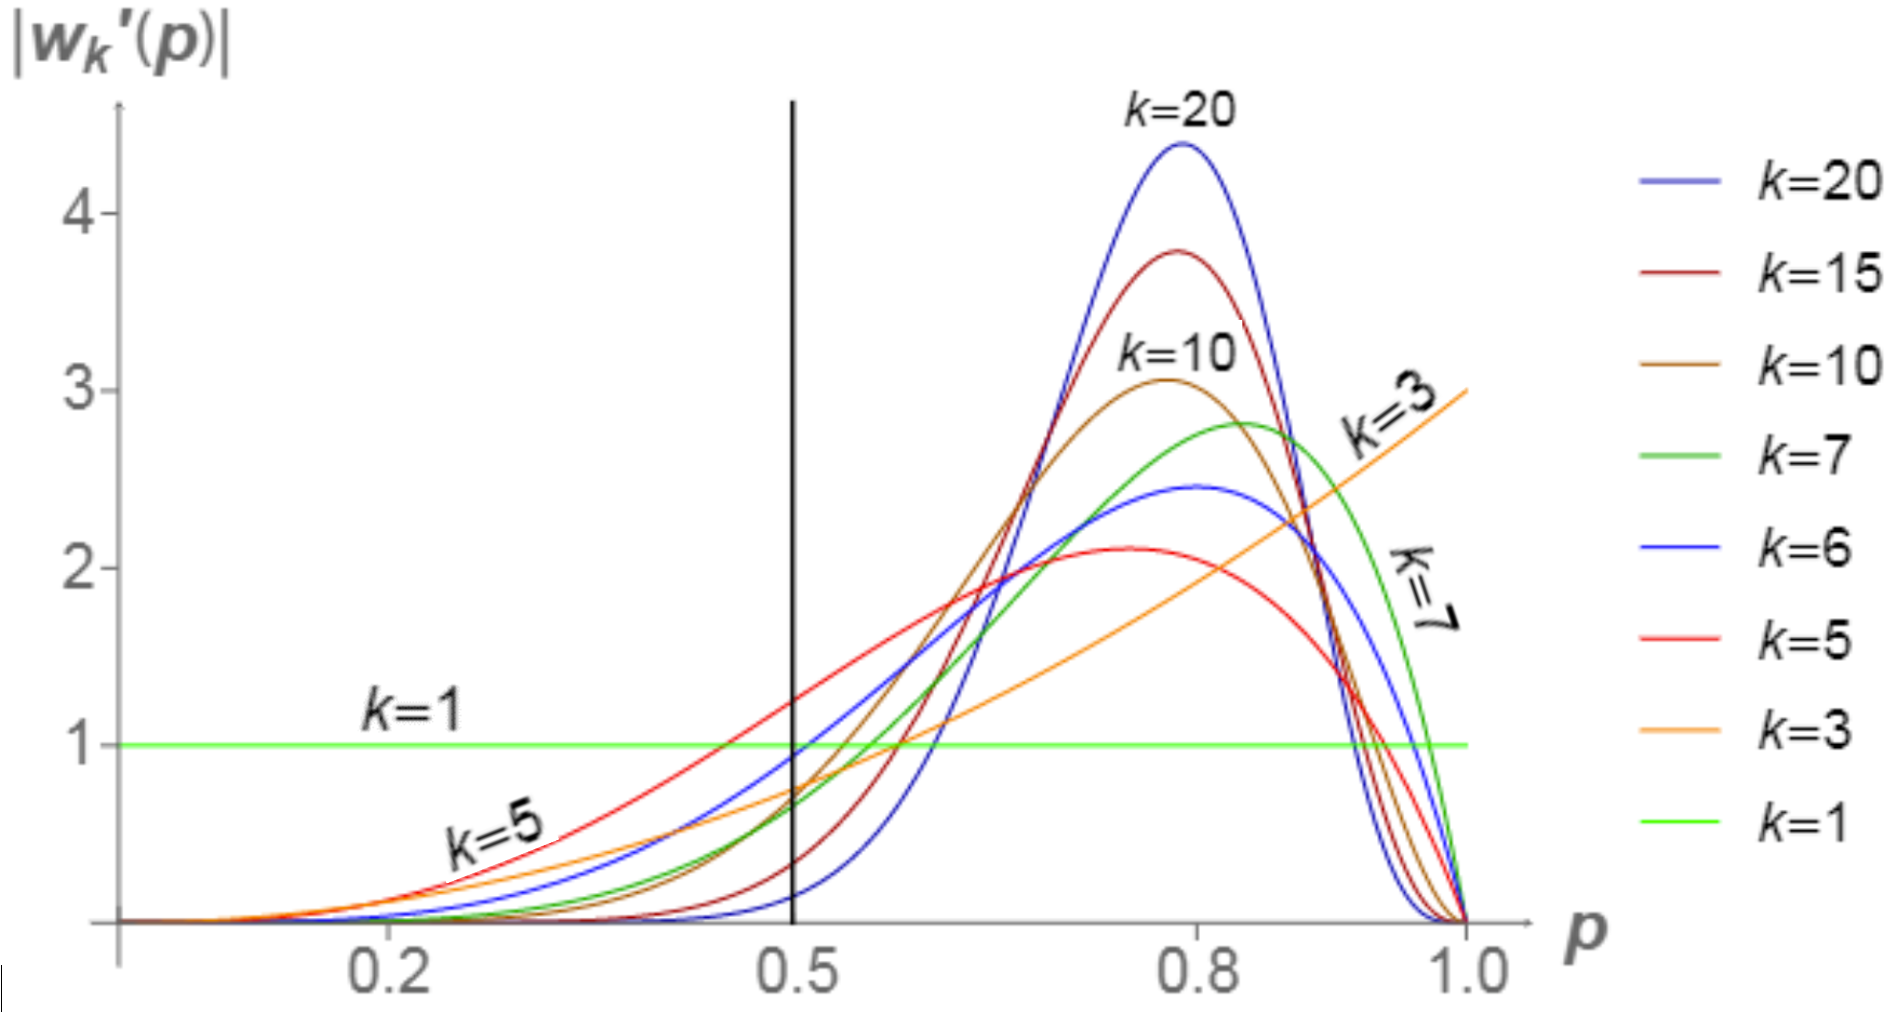
\includegraphics[scale=0.47]{figure2.png}
\label{figure:ASD_stablepicture}
\end{figure} 
%Y(10.5): Should I remove the labels to the right of the figure ?

The function $|w_{\theta}'(p)|$ is a mixture of the functions $|w_k'(p)|$ for the various $k$-s in the support of $\theta_q$ (which are illustrated in Figure \ref{figure:ASD_stablepicture}).
Observe that $|w_1'(p) \equiv 1|$. The formal proof applies the  central limit theorem to show that as $k$ increases, $|w_k'(p)|$ converges  to a normal distribution with mean $\frac{g}{g+l}$ and variance $\frac{1}{4k}.$ The assumption that   $\frac{g}{g+l}\neq \frac{1}{2}$ implies that $|w_k'(0.5)|$ converges to zero. This, in turn, implies that $|w_{\theta_q}'(0.5)|<1$ if $\hat{k}$ is sufficiently large. By continuity, $|w_{\theta_q}'(p^{(\theta_q)})|<1,$ which implies that the symmetric stationary state is asymptotically stable. See Appendix \ref{subsec:stableinterior_ASDproof} for a formal proof. \qedhere

\end{proof}
\subsection{Heterogeneous Populations: An Example}\label{subsec-hetro-action}
Next we demonstrate that heterogeneous populations behave very differently than homogenous populations under that action-sampling dynamics. Specifically, we present an example of a heterogeneous population in which most initial population states converge to a symmetric interior state, even though: (1) most agents have relatively large samples, and (2) the pure stationary states are asymptotically stable.
Consider a population in which $70\%$ of the agents sample 20 actions, while the remaining $30\%$ agent sample two actions (i.e., $\theta(20)=70\%$ and $\theta(2)=30\%$). Consider an underlying game in which the gain of a hawkish player (and the loss of the dovish opponent) is small: $g=l=0.04.$ Figure XXX illustrates the phase plot in this setup. Observe that: (1) the dynamic admits 5 stationary states, (2) three of these states are asymptotically stable: the two pure stationary states and the symmetric stationary state (0.2,0.2),
%Y(22.5): Srinivas please confirm that the stationary state is 0.15
and (3) most initial states converge to the symmetric state (a Monte-Carlo simulation with a uniformly random initial state have converged to the symmetric stationary state in $XXX\%$ of the times.
%Y(22.5): Srinivas, please run such a Monte Carlo simulation and report its result.

%Y(22.5): Srinivas: Please add the phase plot that you made (for \theta(2)=20%) as a figure in the style of figure 1: Axis have no "spare area" (only [0,1], add black/white dots for stable/unsatble states, and try to add \dot(p_2)=0, p_2=w(p_1), \dot(p_1)=0 and p_2=w^-1(p_1) in green/ornage below/above (0.3,0.1).

%Y(22.5): Amnon: Can you please add a one-paragraph intution why all-2 glboally converege to pure, all 20 globally converge to pure, but mix of 2 and 20 converge from most initial states to the symmetric?  


\subsection{Payoff-Sampling
Dynamics\label{subsec:Stability-of-symmetric-payoff-dynamics}}
For tractability in the analysis of payoff-sampling dynamics, we focus on the cases where the gain of a hawkish player and the loss of her dovish opponent are large, namely, $l,g>\frac{1}{\max (\textrm{supp}(\theta))}$. Our result shows that in this domain, the symmetric stationary state 
is asymptotically
stable in the following common cases:
\begin{enumerate}
\item for any homogeneous  distribution of sample sizes $\theta\equiv k<20$; or
\item for any heterogeneous distribution with a maximal sample size of at most 5.
\end{enumerate}
The threshold of $k=20$ is binding. The symmetric stationary state becomes unstable if the sample size is $k \geq 20.$ By contrast, the bound of a maximal size of 5 for heterogeneous distributions of sample sizes is only a constraint of our proof technique. Numeric analysis (see Section \ref{sec:Numeric-Analysis}) suggests that the stability of the symmetric stationary state:
\begin{enumerate}
    \item holds for many distributions of types with larger maximal sample sizes (in particular, it holds for uniform distributions over 
$\left\{ 1,\dots,k\right\} $ for any $k\leq20$); and
    \item is often global (i.e., in many cases almost all initial states converge to this state).
\end{enumerate}
\begin{thm}\label{thm:stableinterior_PSD}
Assume that $l,g\in\left(\frac{1}{\max\left(\emph{supp}(\theta\right))},1\right)$, and either (1) $\theta\equiv k<20$, or (2) $\max\left(\emph{supp}(\theta\right))\leq5.$ Then, the game admits an asymptotically stable symmetric stationary state 
%$\left(p^{(\theta)}, p^{(\theta)}\right)$
under the payoff-sampling dynamics. Moreover, the frequency of two hawks being matched together in this state is at least $25\%$.
\end{thm}
\begin {proof}[Sketch of Proof] When $l$ and $g$ are sufficiently large, the payoff of action $h$ is slightly below twice the number of $d$-s in the $h$-sample, and the payoff of action $d$ is slightly above the number of $d$-s in the $d$-sample. This implies that action $h$ has a higher mean payoff than action $d$ iff the number of $d$-s in the $h$-sample is strictly greater than half the number of $d$-s in the $d$-sample. 
\begin{figure}[h]
\centering
\caption{The Function $w_k(p)$ for Various Values of $k$}
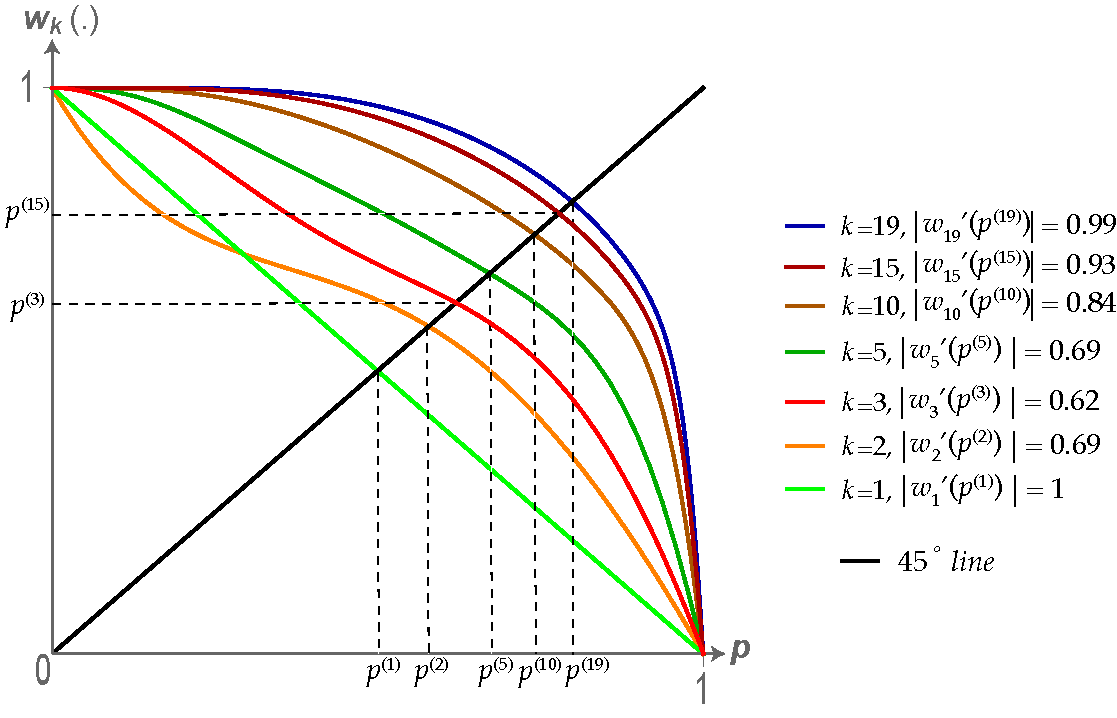
\includegraphics[scale=0.75]{Figures/PSD_stable.pdf}
\label{fig:proofbypicture}
%\label{fig:wkp}
\end{figure}

Thus, we can write $w_k(p)$ as follows:
\begin{equation}\label{eq:wkp-p}
w_{k}(p)=P\left(\underbrace{k-X_{k}(p)}_{\#d_{j}\,\textrm{in}\,h\textrm{\textrm{-}sample}}>\frac{1}{2}\underbrace{(k-Y_{k}(p))}_{\#d_{j}\,\textrm{in}\,d\textrm{-sample}}\right)=P(2X_{k}(p)-Y_{k}(p)<k),
\end{equation}
where $X_k(p)$ and $Y_k(p)$ are iid binomial random variables with parameters $k$ and $p.$ 

In the formal proof (see Appendix \ref{subsec:stableinterior_PSDproof}), we show that for any $k<20,$ $w_k(p)$ has a unique fixed point $p^{(k)}$ such that $|w_k'(p^{(k)})|<1$ (see Figure \ref{fig:proofbypicture}). This implies, by the same argument as in the sketch of proof of Theorem \ref{thm:unstableinterior_ASD}, that the symmetric stationary state is asymptotically stable. (By contrast, one can verify that $|w_k'(p^k)|>1$ for $k \geq 20,$ which implies that the symmetric stationary state is unstable for large $k\geq20$.) 

Next, we verify in the formal proof that for any $k \in \left\{1,2,3,4,5\right\}$ it holds that (I) the fixed points  are all in the interval $(0.5,0.68)$, and  (II) $|w_k'(p)|<1$ for any  $k \in \left\{1,...,5\right\}$ and any $p \in (0.5,0.68).$ Let $\theta$ be any distribution with $\max(\textrm{supp}(\theta)) \leq 5$. The fact that $w_\theta(p)$ is a weighted average of the various $w_k(p)$ implies that  (I) the fixed point $p^{(\theta)}$ of $w_\theta(p)$ is in $(0.5,0.68)$, and (II) $|w_\theta'(p^{(\theta)})|<1$ $\Rightarrow$ $(p^{(\theta)}, p^{(\theta)})$ is asymptotically stable.
\qedhere
\end{proof}



\section{Numeric Analysis\label{sec:Numeric-Analysis}}

We present numeric results that complement
the analytic results of the previous sections. 


\paragraph{Methodology and Parameter Values}

The analysis focuses on the standard hawk--dove games, in which the gain of a hawkish player is equal to the loss of her dovish opponent, i.e., $g=l$
for each $i\in\left\{ 1,2\right\} $. We have tested the following $270=10 \times 27$ combinations of parameter values for each of the two sampling dynamics:
\begin{enumerate}
\item 10 values for $g$: 0.05, 0.15,
0.25, 0.35, 0.45, 0.55, 0.65, 0.75, 0.85, 0.95.
\item 27 distributions of sample sizes:
\begin{enumerate}
\item 9 \emph{degenerate distributions}, in which all agents have sample size $k$,
for each $2\leq k\leq10$ (the case of $k=1$ is discussed in Footnote \ref{foot-k-1}). 
\item 9 \emph{uniform distributions} over $\left\{ 1,..,k\right\} $, for each $2\leq k\leq10$.

\item 9 \emph{$1$-biased distributions},
in which a share $q \in \left\{10\%, 20\%, ..., 90\%\right\}$ of the new agents have sample size one, while the sample sizes of the remaining agents are distributed uniformly over \{1,2,\dots, 10\}. That is, the frequency of sample size 1 is $\frac{1-q}{10} + q$ and the frequency of each $k \in \{2,\dots, 10\}$ is $\frac{1-q}{10}.$ 
\end{enumerate}
\end{enumerate}
For each set of parameters, we have numerically calculated the phase portrait and
the curves for which $\dot{p}{}_{1}=0$ and $\dot{p}{}_{2}=0$, and
used this to determine the dynamic behavior. 
The code is provided in the online supplementary material.\footnote{
Our numeric analysis is based on deterministic dynamics in a continuum population. We have randomly chosen 10 of these combinations of parameter values, and tested each of them by running it 100 times in the stochastic dynamics induced by  a finite population of 1,000 agents, using ABED software (\citealp{izquierdo2019introduction}). The results for finite populations are qualitatively the same.}
\begin{figure}[t]\caption{Summary of Results of the Numeric Analysis}\label{fig:numeric_figure}
\begin{centering}
%~~~~~
\includegraphics[scale=0.57]{Figures/\string"numeric-analysis-results\string".png}
 \end{centering}
\end{figure}
\paragraph{Results}
The numeric results are summarized in Figure
\ref{fig:numeric_figure}. 
The action-sampling dynamics typically yield global convergence to the pure equilibria  (orange shaded region in Figure
\ref{fig:numeric_figure}).  The exceptions are consistent with Proposition \ref{prop:pure-equilbiria-satbility} and Theorem \ref{thm:stableinterior_ASD}. Specifically, the action-sampling dynamics admit (almost) global convergence to the symmetric stationary state (green shaded region) if  (1) most agents have sample size 1, and (2) $g$ is sufficiently far from 0.5. 

The payoff-sampling dynamics typically yield global (or almost global) convergence to either the asymmetric pure equilibria  or the symmetric mixed stationary state, where each kind of convergence holds, roughly, in half of the parameter combinations. Global convergence to the symmetric mixed stationary state occurs for all parameter values for which it occurs under the action-sampling dynamics. In addition, the payoff-sampling dynamics globally converge to the symmetric mixed stationary state for all distributions of types, provided that $g$ is sufficiently close to one. 


\section{Conclusion}\label{sec:conclusion}
A key result in evolutionary game theory is that two populations that are matched to play a hawk--dove game converge to one of the pure equilibria from almost any initial state. We demonstrate that this result crucially depends on the revision dynamics being monotone. Specifically, we show that two plausible classes of  dynamics, in which new agents base their chosen actions on sampling the actions of a few agents in the opponent population (action-sampling dynamics) or on sampling the payoffs of a few agents in their own population (payoff-sampling dynamics) can lead to the opposite prediction: global convergence to a mixed stationary state. 


%Y(6.5): I have rephrased the coming first half of the sentence due to R3; instead of explainign it, we just provide a new (or perhaps a novel?) explanation
Our results provide a new explanation why in bargaining situations, such as the motivating example of buying and selling houses, players in both populations tend to play hawkish strategies, and bargaining frequently fails.
Our model assumes that all players in each population have the same payoff matrix. Heterogeneity in the payoffs, and private information regarding one's payoff, are important aspects of many real-life bargaining situations. An interesting direction for future research is to apply the analysis of sampling dynamics in more complicated models that incorporate heterogeneous payoffs.  

\appendix

\section{Appendix\label{sec:Technical-Proofs}}
\subsection{Standard Definitions of Dynamic Stability}\label{sub-standard-definitions}
%Y(8.5): I have moved this subsection to an appendix, as suggested by R2.
For completeness, we present in this appendix  the standard definition of dynamic stability that are used in the paper (see, e.g., \citealp[Chapter 5]{weibull1997evolutionary}).

A state is said to be 
stationary if
it is a rest point of the dynamics.
\begin{defn}
\label{def:equilbirium}State $\mathbf{p}^{*}\in\left[0,1\right]^{2}$
is a \emph{stationary state}
if $w_{i}\left(\mathbf{p}^{*}\right)=p_{i}^{*}$
for each $i\in\left\{ 1,2\right\}$.
\end{defn}
Let $\mathcal{E}\left(w\right)$ denote the set of stationary states of $w,$ i.e., $\mathcal{E}\left(w\right) = \{\mathbf{p}^{*} | w_{i}\left(\mathbf{p}^{*}\right)=p_{i}^{*}\}.$ Under monotone dynamics,  an interior (mixed) state $\mathbf{p}^*\in (0,1)^2$ is a stationary state iff it is a Nash equilibrium (\citealp[Prop. 4.7]{weibull1997evolutionary}). By contrast, under nonmonotone dynamics (such as the sampling dynamics analyzed below) the two notions differ.

A state is Lyapunov stable if a population beginning near it remains close, and it is asymptotically stable if, in addition, it eventually converges to it. A state is
unstable if it is not Lyapunov stable. It is well known (see, e.g., \citealp[Section 6.4]{weibull1997evolutionary})
that every Lyapunov stable state must be a stationary state. Formally:

\begin{defn}
\label{def:lyaponouv-stability} A stationary state $\mathbf{p}^{*}\in\left[0,1\right]^{2}$
is \emph{Lyapunov stable} if for every neighborhood $U$ of $\mathbf{p}^{*}$
there is a neighborhood $V\subseteq U$ of $\mathbf{p}^{*}$ such that if the
initial state $p\left(0\right)\in V$, then $\mathbf{p}\left(t\right)\in U$
for all $t>0$. A state is \emph{unstable} if it is not
Lyapunov stable.
\end{defn}

\begin{defn}
A stationary state $\mathbf{p}^{*}\in\left[0,1\right]^{2}$
is \emph{asymptotically stable} if it is Lyapunov stable and there is some neighborhood $U$
of $\mathbf{p}^{*}$ such that all trajectories initially in $U$ converge
to $\mathbf{p}^{*},$ i.e., $\mathbf{p}\left(0\right)\in U$ implies $\lim_{t\rightarrow\infty}\mathbf{p}\left(t\right)=\mathbf{p}^{*}$.
\end{defn}

%S(9.5): Added the following subsection which rules out limit cycles in planar systems)
%Y(12.5): I tentatively removed it (and it is mentioned only in a footnote in the main text).
%\subsection*{The Bendixson Dulac Theorem}
%The following Theorem (see Theorem 9.A.6 of \cite{sandholm2010population}) known as Bendixson-Dulac Theorem provides a sufficient condition for ruling out the existence of limit cycles in planar systems.
%\begin{thm}\label{thm:BD_thm}
%Let $V: \mathbb{R}^2 \rightarrow \mathbb{R}^2$ be $C^1,$ and consider the differential equation $\dot{x} = V(x).$ If $\text{div} \ V \neq 0$ i.e., $\frac{\partial V}{\partial x_1} + \frac{\partial V}{\partial x_2} \neq 0$ throughout the simply connected set $Y,$ then $Y$ does not contain a closed orbit.
%\end{thm}

%S(9.5): I think applying the above theorem to our dynamics will rule put the existence of limit cycles and therefore only the rest points will be candidates for long term behavior (?) Applying the above theorem in what follows.

%Ignoring the constant $\delta,$ our sampling dynamics can be written as $\dot{p}_1 \equiv V_1(p_1,p_2) = w(p_2) - p_1$ and $\dot{p}_2 \equiv  V_2(p_1,p_2) = w(p_1) - p_2.$ Clearly, $\text{div} \ V  = \frac{\partial V}{\partial p_1} + \frac{\partial V}{\partial p_2} = -2 \neq 0.$ Thus, there are no limit cycles.

%Yׂׂ(9.5): Is the assumption o fthe set Y being simply connnected innocent? Does the theorem rules out a trjactory that converges to a limit cycle? (but it is not a cycle itself?)
%Does the conditions imply convergence of any trjactory to stationary states?


\subsection{Proof of Proposition \ref{pro-convergence-to-stationary} (Convergence to Stationary States) %Properties
}\label{proof-convergence-to-stationary}
%Y(13.5): New paragraph to formally define above/below/right/left
We say that state $\textbf{p}$ is \emph{above} (resp., \emph{below}) curve $w(p_1)$ if $p_2>w(p_1)$ (resp., ($p_2<w(p_1)$). Similarly, we say that state $\textbf{p}$ is to the \emph{right} (resp., \emph{left})  of the curve $w(p_1)$ if $w^{-1}(p_2)<p_1$ (resp., $w^{-1}(p_2)<p_1$). We say that the state $\textbf{p}$ is on the curve $w(p_1)$ if $p_2=w(p_1).$

The fact that the two curves of $w(p_1)$ and $w^{-1}(p_1)$ are strictly decreasing implies that a state is above one of these curves iff it is to the right of that curve. The states on the curve $w(p_1)$ (resp., $w^{-1}(p_1)$) are characterized by having $\dot{p_1}=0$ (resp., $\dot{p_2}=0$). Observe that in any state $\textbf{p}$ above and to the right (resp., below and to the left) of the curve $w(p_1)$, the share of hawks in the population 2 is higher relative to the corresponding state on the curve with the same share of hawks in population 1, implies that $\dot{p_1}<0$ (resp., $\dot{p_1}>0$). Similarly, in any state $\textbf{p}$ above (resp., below) the curve $w^{-1}(p_1)$, the  share of hawks in population 1 is higher relative to the corresponding state on the curve with same share of hawks in population 2, which implies that $\dot{p_1}<0$ (resp., $\dot{p_1}>0$).

Any state $\textbf{p}\in[0,1]$ can be classified in one of 3*3 classes, depending on its relative location WRT the two curves, i.e., whether $\textbf{p}$ is below (=to the left of), above (=to the right of) or on the curve $w(p_1)$, and similarly whether $\textbf{p}$ is below, above or on the curve $w^{-1}(p_1)$. 
The above argument implies that this classification determines the signs of $\dot {p_1}$ and $\dot {p_2}$. If state $\textbf{p}$ is on (resp., above, below) the curve $w(p_1)$, then $\dot {p_2}$ is zero (resp., negative, positive). Similarly, if state $\textbf{p}$ is on (resp., above, below) the curve $w^{-1}(p_1)$, then $\dot {p_1}$ is zero (resp., negative, positive).

In particular, any state  $\textbf{p}$ that is above (resp., below) both curves must satisfy that $\dot {p_1},\dot {p_2}$ are both negative (resp., positive). This implies that any trajectory that begins  above (resp., below) both curves (namely, $w(p_1)$ and $w^{-1}(p_1)$) must always move downwards and to the left. This (together with the fact that all stationary states are in the intersection of the two curves) implies  that the trajectory must cross one of the curves. If this crossing point is an intersection of both curves, then it is a stationary state.

Next observe that any trajectory that starts on one of the curves and strictly above (resp., below) the remaining curve must move to a state that is strictly below one of the curves and strictly above the remaining curve. This is so because on the crossing point one of the $\dot {p_i}$ is zero and the remaining derivative $\dot{p_j}$ is negative (resp., positive), which implies that the trajectory must move below and to the left (resp., above and to the right) of the curve that was crossed.

Thus, we have established that any trajectory (which have not converged to a stationary state) must reach a state that is strictly below one of the curves and strictly above the remaining curve. If such a state is strictly above the curve $w(p_1)$, then by the classification mentioned above the trajectory must move both downward and to the right; i.e., $\dot{p_1},\dot{p_2}<0$ (resp., both upward and to the left; i.e., $\dot{p_1},\dot{p_2}>0$). This implies that the trajectory must cross one of the curves. The crossing point cannot be only on the curve of $w(p_1)$ (resp., $w^{-1}(p_1)$, because in such a point the trajectory moves horizontally to the left (vertically downward), which implies that it must cross the lower (resp., higher)  curve $w(p_1)$ (resp.,$w^{-1}(p_1)$) from the left side (resp., from above) and we get a contradiction. The argument in case the state is strictly below rhe curve $w(p_1)$ is analogous.
 
%Y(9.5): New formal proof. A & S, please read carefully, and improve the rigrousness, if required.
\subsection{Proof of Proposition \ref{pro-convergence-to-pure-iff-asymp} (Convergence to Pure Equilibria)}\label{proof-converge-pure-iss-asymp}
 If $\textbf{p}$ is below  (resp., above) both curves, then by the classification presented above it must that $\dot{p_1}>0$ (resp., $\dot{p_2}<2$), which implies (by a similar argument to the proof of Proposition \ref{pro-convergence-to-stationary}) that convergence to (1,0) is possible only if the trajectory passes through a state that is strictly between the two curves, and that the closest intersection point of the two curves to the left of this state is (1,0). By the classification presented above it must that the curve of $w^{-1}(p_1)$ is strictly below the curve of $w(p_1)$ in a right neighborhood of (1,0), which implies that (1,0) is asymptotically stable because any sufficiently close initial state would converge to (1,0)
\subsection {Proof of Lemma \ref{lemma-sample} (Maximal Sample Sizes)}\label{lem-proof}

\begin{enumerate}
\item (I) The sum of payoffs of action $h$ (resp., $d$) against
a sample with a single $d$ is $1+g$ (resp., $1+\left(k-1\right)(1-l)$).
The mean payoff of $h$ is strictly higher than 
the mean payoff of $d$ iff
%Y(9.5): removed the footnote: \footnote{A tie between the two samples is impossible due to Assumption \ref{asu:generic} of having a generic environment.}
$k<\frac{1+g-l}{1-l}.$
(II) The sum of payoffs of action $d$ (resp., $h$) against
a sample with a single $h$ is $k-1+1-l$ (resp., $\left(k-1\right)\left(1+g\right)$).
The mean payoff of $h$ is higher than 
the mean payoff of $d$ iff $k<\frac{1+g-l}{g}$. 
\item (I) The sum of payoffs of a $h$-sample with a single $d$ is equal to $1+g$. The sum of payoffs of a $d$-sample with no $d$ is equal to $k\cdot l$. The former sum is
higher than the latter iff $k<\frac{1+g}{1-l}.$
(II) The sum of payoffs of a $d$-sample with no $h_{j}$-s is
equal to $k$. The sum of payoffs of an $h$-sample with a single
$h_{j}$ is equal to $(k-1)\left(1+g\right)$. The former sum
is higher than the latter iff $k<\frac{1+g}{g}$.\qedhere
\end{enumerate}




\subsection {Proof of Proposition \ref{prop:pure-equilbiria-satbility} (Stability of Pure Equilibria)}\label{subsec:Proof-of-Theorem-2}
We are interested in deriving conditions for the stability of the pure stationary states. 
In what follows,
we compute the Jacobian of the sampling dynamics at the state 
%Y(6.5): I have revised the following sentences till the end of the paragraph, removing (0,1), as sugegsted by referee 2.
in which all agents of population $i$ play $d$ and all agents of population $j$ play $h$. For this, we consider a slightly perturbed state with a ``very small'' $\epsilon_i$ share of hawks in population $i$ and a ``very small'' $\epsilon_j$ share of doves in population $j.$ By ``very small,'' we mean that higher-order terms of $\epsilon_i$ and $\epsilon_j$ are neglected.

 Consider a new agent of population
$i$ with a sample size of $k_{i}.$ Action $h$ has a higher mean
payoff against a sample size of $k_{i}$ iff (neglecting rare events
of having multiple $d$-s in the sample): (1) the sample includes the single action $d$ of an opponent, and (2) $k_{i}\leq m_{h}$
 (due to Lemma \ref{lemma-sample}). The probability of (1) is $k_{i}\cdot\epsilon_{j}+o(\epsilon_{j})$,
where $o(\epsilon_{j})$ denotes terms that are sublinear in $\epsilon_{j}$,
and, thus, it will not affect the Jacobian as $\epsilon_{j}\rightarrow0$.
This implies that the probability that a new agent of population $i$
(with a random sample size distributed according to $\theta$)
has a higher mean payoff for action $h$ against her sample is
$w_{\theta}(1-\epsilon_{j})=\epsilon_{j}\cdot\sum_{k_{i}=1}^{m_{h}}\theta(k_i)\cdot k_{i}+o(\epsilon_{j})$.
An analogous argument implies that the probability that a new agent
of population $j$ has a higher mean payoff for action $d_{j}$ against
her sample is $w_{\theta_{j}}(\epsilon_{i})=\epsilon_{i}\cdot\sum_{k_{j}=1}^{m_{d}}\theta_{j}(k_j)\cdot k_{j}+o(\epsilon_{i})$.
Therefore, the sampling dynamics at $(\epsilon_{i},1-\epsilon_{j})$
can be written as follows (ignoring the higher-order terms
of $\epsilon_{i}$ and $\epsilon_{j}$):
\begin{equation}
\dot{\epsilon}_{i}=\epsilon_{j}\cdot\sum_{k_{i}=1}^{m_{h}}\theta(k_i)\cdot k_{i}-\epsilon_{i},\,\,\,\,\,\,\,\,\,\,\,\,\dot{\epsilon}_{j}=\epsilon_{i}\cdot\sum_{k_{j}=1}^{m_{d}}\theta_{j}(k_j)\cdot k_{j}-\epsilon_{j}.\label{eq:a_b_theta}
\end{equation}
Define: $a_{\theta}=\sum_{k_{i}=1}^{m_{h}}\theta(k_i)\cdot k_{i}$
and $b_{\theta}=\sum_{k_{j}=1}^{m_{d}}\theta_{j}(k_j)\cdot k_{j}$.
The Jacobian of the above system of Equations \eqref{eq:a_b_theta}
is then given by $J=\left(\begin{array}{cc}
-1 & a_{\theta}\\
b_{\theta} & -1
\end{array}\right).$ The eigenvalues of $J$ are $-1-\sqrt{a_{\theta}b_{\theta}}$
and $-1+\sqrt{a_{\theta}b_{\theta}}.$ Observe that:
(1) if $a_{\theta}b_{\theta}<1$ then both eigenvalues
are negative, which implies that the state in which
%Y(6.5): I slightly rephrased the following end of sentence to remove the notation (f,h) due to referee 2's comment.
all agents in population $i$ (resp., $j$) are doves (resp., hawks) is asymptotically
stable, and (2) if $a_{\theta}b_{\theta}>1$ then
one of the eigenvalues is positive, which implies that this state is unstable (see, e.g., \citealp[Theorems 1--2 in Section 2.9]{perko2013differential}).

%Y(6.5): New short proof due to Referee 2's comment that Corollary 2 is not immediate. Please check.
\subsection{Proof of Corollary \ref{cor:g=l}\label{proof-cor-g=l} (Standard Case of $g=l$)}
Substituting $g=l$ in  the bounds presented in Definition \ref{def:maximal-samples} yields the following bounds: 
 $\,m_{h}^{A}=\left\lfloor \frac{1}{1-g}\right\rfloor ,\,m_{d}^{A}=\left\lfloor \frac{1}{g}\right\rfloor,
 m_{h}^{P}=\left\lfloor \frac{1+g}{1-g}\right\rfloor ,\,m_{d}^{P}=\left\lfloor \frac{1+g}{g}\right\rfloor.$
 Observe that $\min(m_{h}^{A},m_{d}^{A})=\min( \frac{1}{1-g}, \frac{1}{g})=1$. This implies that  
 $\mathbb{E}_{\leq m_{h}^A}\left(\theta\right)\cdot \mathbb{E}_{\leq m_{d}^A}\left(\theta\right)=\theta(1)\cdot\mathbb{E}_{\leq \max\left(\frac{1}{g},\frac{1}{1-g}\right)}\left(\theta\right),$ which proves part 1.
 Next observe that if $g<\frac{1}{3}$, then  $\min(m_{h}^{P},m_{d}^{P})=\min(\frac{1+g}{1-g},\frac{1+g}{g})=1$ and $\max(m_{h}^{P},m_{d}^{P})=\max(\frac{1+g}{1-g},\frac{1+g}{g})=\frac{1+g}{g}$, which proves part (2-a). Finally, observe that if $g\geq\frac{1}{3}$, then 
 $\min(m_{h}^{P},m_{d}^{P})=\min(\frac{1+g}{1-g},\frac{1+g}{g})=2$ and $\max(m_{h}^{P},m_{d}^{P})=\max(\frac{1+g}{1-g},\frac{1+g}{g})=\max(3,\frac{1+g}{1-g})$, which proves part (2-b).
 
\subsection{Proof of Theorem \ref{thm:unstableinterior_ASD} (Homogeneous Populations, ASD)}\label{subsec:unstableinterior_ASDproof}
Recall that the action-sampling dynamics in state $(p_1,p_2)$ are given by
\begin{equation}\label{eq:Jacobsystem_ASD}
    \dot{p}_1 = \delta(w_k(p_2) - p_1) \hspace{0.3in} \text{and} \hspace{0.3in}
    \dot{p}_2  = \delta(w_k(p_1) - p_2),
\end{equation}
where, for brevity we omit the superscript A, i.e., we write $w_k \equiv w^A_k.$

Observe that a symmetric state $(r,r)$ 
is a stationary state of the dynamics iff $r$ is a fixed point of the function $w_k(p).$ Let $X_k(p)$ denote a binomial distribution with parameters $k$ and $p.$ Let  $m = \left\lfloor \frac{kg}{1+g-l}\right\rfloor.$ Note that the possible values of $m$ are $\{0,1,\dots,k-1\}.$ To make the dependence of the function $w_k(p)$ on $m$ explicit, we write as follows:
\begin{equation}\label{eq:wkmp}
w_k(p) \equiv w_{k,m}(p)= P(X_k(p) \leq m) = F(m;k,p),
\end{equation}
where $F(\cdot \ ;k,p)$ is the cumulative distribution function of a binomial distribution with parameters $k$ and $p.$ For all $m,$ it follows that $w_{k,m}(0)=1, w_{k,m}(1) =0,$ and $w_{k,m}(p)$ is decreasing in $p,$ which implies that $w_{k,m}(p)$ has a unique interior fixed point $p^{(m)}.$ 

In order to assess the asymptotic stability, we compute the Jacobian $J$ of 
Eq. \eqref{eq:Jacobsystem_ASD} at the symmetric rest point $(p^{(m)}, p^{(m)})$ 
(ignoring the constant $\delta$, which plays no role in the dynamics, except multiplying the speed of convergence by a constant): 
$$
J =  \left( \begin{array}{cc}
-1 & w'_{k,m}(p^{(m)})  \\
w'_{k,m}(p^{(m)}) & -1  \end{array} \right).
$$
The eigenvalues of $J$ are $-1+w'_{k,m}(p^{(m)})$ and $-1-w'_{k,m}(p^{(m)}).$ A sufficient condition for instability at $(p^{(m)}, p^{(m)})$ is that $|w'_{k,m}(p^{(m)})| > 1.$ 

From Eq. \eqref{eq:wkmp}, we now compute as follows:
\begin{align*}
    w_{k,k-m-1}(1-p)+w_{k,m}(p) &= P(X_k(1-p) \leq k-m-1) + P(X_k(p) \leq m)\\
    &= P(X_k(p) \geq k-(k-m-1)) + P(X_k(p) \leq m) \\
    &= P(X_k(p) \geq m+1) + P(X_k(p) \leq m) = 1.
\end{align*}
The fact that  $ w_{k,k-m-1}(1-p)=1-w_{k,m}(p)$ implies that $p^{(k-m-1)} = 1 - p^{(m)}$ and $w_{k,k-m-1}'(p^{(k-m-1)}) = w_{k,m}'(p^{(m)}).$ Without loss of generality, we can therefore focus on analyzing the cases of $m$ for which $m \leq \left\lfloor \frac{k-1}{2}\right\rfloor.$ To ease notation, we fix $k\geq 2$ and define a new function $f_m:[0,1] \rightarrow [0,1]$ as $f_m(p) \equiv w_{k,m}(p)$ and let $r_m = p^{(m)}$ be the fixed point of the function $f_m(p),$ i.e., $f_m(r_m) = r_m.$ Since $f_m(0) = 1,$ $f_m(1) = 0,$ and $f_m(\cdot)$ is a strictly decreasing function, it follows that the fixed point $r_m \in (0,1)$ and that it is unique. 
To complete the proof we need to show that $|f_m'(r_m)| > 1$ for nonnegative integer values of $m$ such that $m \leq \frac{k-1}{2}.$ In what follows, we show this. 

It is well known (see, e.g., \citealp{green1983fixed}) that
\[f_{m}(p)\equiv w_{k,m}(p) = \sum_{i=0}^{m}\binom{k}{i}p^i(1-p)^{k-i} = \binom{k}{m}(k-m)\int_{0}^{1-p}t^{k-m-1}(1-t)^m dt.\]
We now compute as follows:
\begin{align}\label{eq:wkmprime}
    f_{m}'(p) &= -\binom{k}{m}(k-m)p^m(1-p)^{k-m-1} = -k\binom{k-1}{m}p^m(1-p)^{k-m-1}\\
    f_{m}''(p) &= \binom{k}{m}(k-m)p^{m-1}(1-p)^{k-m-2}((k-m-1)p-m(1-p)).\nonumber
\end{align}
Fix an $m$ such that $1 \leq m\leq \left\lfloor \frac{k-1}{2}\right\rfloor.$ From the above computations, it follows that the function $f_{m}(p)$ is concave for values of $p \leq p^{\ast}$ and convex for values of $p \geq p^{\ast}$ where $p^{\ast} = \frac{m}{k-1}.$ This is because $f_m''(p^{\ast}) =0.$ Either the concave part or the convex part of the function $f_{m}(p)$ intersects the $45^{\text{o}}$ line. Suppose that the concave part of the function $f_{m}(p)$ intersects the $45^{\text{o}}$ line from the origin, i.e., $r_m \leq \frac{m}{k-1}.$ In this case, $f_{m}(p)$ intersects the $-45^{\text{o}}$ line joining the points (1,0) and (0,1) at $q^{\ast},$ where $q^{\ast}<r_m.$ This is because $m \leq \left\lfloor \frac{k-1}{2}\right\rfloor$ implies that $r_m \leq 0.5$ as $f_{m}(0.5) \leq 0.5$ for such values of $m.$ Since the function $f_{m}(p)$ intersects the $-45^{\text{o}}$ line from above, we can conclude that $f_{m}'(q^{\ast}) <-1.$ The function $f_{m}(p)$ is concave between $q^{\ast}$ and $r_m;$ therefore, we have $f_{m}'(r_m) < f_{m}'(q^{\ast}) < -1,$ i.e., $|f_{m}'(r_m)| >1.$ Therefore we are done in cases where $r_m \leq \frac{m}{k-1}.$

If the convex part of the function intersects the $45^{\text{o}}$ line from the origin, then $r_m > m/(k-1).$ By definition, we have
\begin{align}
   %f_m(p) &\equiv w_{k,m}(p) = (1-p)^k + \binom{k}{1}p(1-p)^{k-1} + \dots + \binom{k}{m}p^m(1-p)^{k-m}\\
   r_m &= (1-r_m)^k + \binom{k}{1}r_m(1-r_m)^{k-1} + \dots + \binom{k}{m}r_m^m(1-r_m)^{k-m}\label{eq:fixedpointpm}
\end{align}
For $j = 0,1,2,\dots,m,$ let $a_j$ denote the $j^{\text{th}}$ term of the sum on the RHS of Eq. \eqref{eq:fixedpointpm}. For $j = 1,2,\dots, m,$ we compute as follows:
\begin{align*}
    &\frac{a_j}{a_{j-1}} = \frac{\binom{k}{j}r_m^j(1-r_m)^{k-j}}{\binom{k}{j-1}r_m^{j-1}(1-r_m)^{k-j+1}}=\left(\frac{k-j+1}{j}\right)\left(\frac{r_m}{1-r_m}\right)\\
    &\frac{a_j}{a_{j-1}}\geq 1 \iff (k-j+1)r_m \geq j(1-r_m) \iff r_m \geq \frac{j}{k+1}.
\end{align*}
Since $\frac{m}{k-1} > \frac{j}{k+1}$ for $j =1,2,\dots, m,$ we have $r_m \geq \frac{j}{k+1}$ and thus $a_j \geq a_{j-1}$. This implies that $a_j \leq a_m$ for $j=1,2\dots,m-1.$ From Eq.\eqref{eq:fixedpointpm}, we can thus conclude the following:
\begin{equation}\label{eq:fixedpointinequality}
    r_m \leq (m+1)\binom{k}{m}r_m^m(1-r_m)^{k-m}.
\end{equation}
From Eqs. \eqref{eq:wkmprime} and \eqref{eq:fixedpointinequality}, we have
\[
|f_m'(r_m)| = (k-m)\binom{k}{m}r_m^m(1-r_m)^{k-m-1} \geq \left(\frac{k-m}{m+1}\right)\frac{r_m}{1-r_m}.
\]
From the above set of equations, a sufficient condition for $|f_m'(r_m)| > 1$ can be written as follows:
\begin{equation}\label{eq:suffcondmodgeq1}
\left(\frac{k-m}{m+1}\right)\frac{r_m}{1-r_m} > 1 \iff r_m > \frac{m+1}{k+1}.
\end{equation}
We will now establish that $|f_m'\left(\frac{m+1}{k+1} \right)| > 1.$ From Eq. \eqref{eq:wkmprime}, we have
\begin{align*}
    |f_m'(p)| &= k\binom{k-1}{m}p^m(1-p)^{k-m-1} = k\cdot \Pr (X_{k-1}(p) = m).
\end{align*}
where $X_{k-1}(p)$ is a binomial distribution with parameters $k-1$ and $p.$ It is a known fact that the binomial distribution's mode with parameters $k-1$ and $p$ is attained at $\lfloor kp \rfloor.$ For $p = \frac{m+1}{k+1},$ we have 
\[
m \leq  k\cdot \left(\frac{m+1}{k+1}\right)  < m+1.
\]
The above inequalities imply that 
$\left \lfloor k\cdot \left(\frac{m+1}{k+1}\right) \right \rfloor = m.$ The binomial distribution $X_{k-1}(\cdot)$ has $k$ possible values and thus the probability of the occurrence of the mode has to be greater than $\frac{1}{k},$ i.e.,
\[
\Pr\left(X_{k-1}\left(\frac{m+1}{k+1}\right)= m \right) > \frac{1}{k} \implies \left|f_m'\left(\frac{m+1}{k+1} \right)\right| > 1.
\]
We need to consider the following two possible cases:

\textbf{Case 1:} $\frac{m}{k-1} < r_m \leq \frac{m+1}{k+1}$. 
For $1\leq m \leq \frac{k-1}{2},$ we know that $|f_m'(\cdot)|$ attains its maximum value at $\frac{m}{k-1}$ and that it is strictly decreasing for $p > \frac{m}{k-1}.$ For $m=0,$ $|f_m'(\cdot)|$ is strictly decreasing for $p>0.$ Thus, we have:
\[
|f_m'(r_m)| > \left|f_m'\left(\frac{m+1}{k+1} \right)\right| > 1.
\]

\textbf{Case 2:} $r_m > \frac{m+1}{k+1}.$ Here, we are done by the sufficient condition of Eq. \eqref{eq:suffcondmodgeq1}.
Next we are left with showing that the dynamics do not admit non-symmetric stationary states.
%Y(22.5): Amnon please add here your formal proof

\subsection{Proof of Theorem \ref{thm:stableinterior_ASD} (Stable Symmetric State: ASD)}\label{subsec:stableinterior_ASDproof}
Let $a = \frac{g}{1+g-l}.$ Under the assumption of generic environment, $a \neq \frac{1}{2}.$ From Eq. \eqref{eq:wkmprime}, we have
\[
|w_{k,m}'(p)|\equiv|f_m'(p)|=k\binom{k-1}{m}p^{m}(1-p)^{k-m-1}\Rightarrow|w_{k,m}'(p)|=k\cdot\Pr\left(X_{k-1}=m\right),
\]
where $m = \lfloor ka\rfloor$ and $X_{k-1}\sim Bin\left(k-1,p\right).$ 

Our first step is to show that if $p=0.5$ then $|w_{k,m}'(p)|$ converges to zero as $k$ goes to infinity. So let $V$ be a sequence defined by: $V_k=k\cdot\Pr\left(X_{k-1}=m\right)$, and $p=0.5$. We assume that $a$ is a rational number,\footnote{If $a$ is irrational, we can apply the same method of proof by taking a rational number that is close enough to $a$.} and specifically, $a=n_1/n_2$, where $n_1$ and $n_2$ are integers. By assumption, $a<1$, and therefore $n_1<n_2$. Our strategy is to divide $V$ into $n_2$ disjoint subsequences whose union is exactly $V$, and show that each one of them convergences to zero. This completes the proof that $V$ convergences to zero.

We define these subsequences as follows: for each value of $i\in \{1,...\,n_2\}$, the elements of a subsequence $V^i$ are $V^i_k=V_{i+k\cdot n_2}$. We would like to show that for each such $i$,
\[
\lim_{k\rightarrow\infty}\frac{V^i_k}{V^i_{k+1}}=\lim_{k\rightarrow\infty}\prod_{j=0}^{n_2-1}\frac{V_{i+k\cdot n_2+j}}{V_{i+k\cdot n_2+j+1}}< 1.
\]
Let $m$ and $j$ be two integers, and let
\[
U_{m+j}\equiv \frac{V_{m+j}}{V_{m+j+1}}=\frac{(m+j)\binom{m+j-1}{\lfloor(m+j)a\rfloor}0.5^{m+j-1}}{(m+j+1)\binom{m+j}{\lfloor(m+j+1)a\rfloor}0.5^{m+j}}.
\]

Given some integer $m$, let $$S=\bigg\{\lfloor(m+j+1)a\rfloor-\lfloor(m+j)a\rfloor\bigg|j\in \{1,2,...\ ,n_2\}\bigg\}$$ 
be a sequence of $n_2$ numbers, and note that $S$ contains only zeros and ones. We claim that $S$ contains $n_1$ ones and $n_2-n_1$ zeros. To see this, 
 given two integers $n_1<n_2$, consider a sequence of $n_2+1$ integers ordered by size, whose set of values contains all integers between some integer $m$ and $m+n_1$, included (so the sequence contains $n_1+1$ different values, with some duplicates). 
Now consider the sequence of differences between any two adjacent numbers of the first sequence.
The latter sequence contains $n_2$ elements, with $n_1$ of them equal to one, and $n_2-n_1$ of them equal to zero. The sequence $S$ can be defined exactly this way. Indeed, for values of $j$ in $(1,2,...\ ,n_2,n_2+1)$, the expression $\lfloor(m+j)a\rfloor$ takes each value between $\lfloor(m+1)a\rfloor$ to $\lfloor(m+n_2+1)a\rfloor$, i.e., $n_1+1$ different values, and the $n_2$ elements of $S$ are exactly the difference between each two adjacent elements. 

For values of $j$ for which the corresponding value in $S$ is zero we have
\[
U_{m+j}=2\frac{m+j}{m+j+1}\cdot \frac{\lfloor(m+j+1)a\rfloor}{m+j}=2\frac{\lfloor(m+j+1)a\rfloor}{m+j+1},
\]
and when the corresponding value is one we have
\[
U_{m+j}=2\frac{m+j}{m+j+1}\cdot \frac{m+j+1-\lfloor(m+j+1)a\rfloor}{m+j}=2\frac{m+j+1-\lfloor(m+j+1)a\rfloor}{m+j+1}.
\]

Since $\lim_{m\rightarrow\infty}\frac{\lfloor(m+j+1)a\rfloor}{m+j+1}=a$ and $\lim_{m\rightarrow\infty}\frac{m+j+1-\lfloor(m+j+1)a\rfloor}{m+j+1}=1-a$, we have 
\begin{align*}
\lim_{k\rightarrow\infty}\frac{V^i_k}{V^i_{k+1}}=\lim_{k\rightarrow \infty}\prod_{j=0}^{n_2-1}U_{i+k\cdot n_2+j}&=2^{n_2}\cdot a^{(1-a)\cdot n_2}\cdot (1-a)^{a\cdot {n_2}}\\
&=\bigg(2\cdot a^{1-a}\cdot (1-a)^{a}\bigg)^{n_2}<1.
\end{align*}
It is smaller than one because the function $a^{1-a}\cdot (1-a)^{a}$ takes its maximum at $a=0.5$, where its value is $0.5$. By the assumption of a generic environment, $a\neq 0.5$. This completes the first stage of the proof.

The first step implies that there is $\hat{k}$ such that $|w_{k}'(0.5)|<0.5$ for any $k\geq\hat{k}$. By continuity, there exists $\epsilon>0$, such that $|w_{k}'(p)|<1$ for any $p\in\left[0.5-\epsilon,0.5+\epsilon\right]$
and any $k\geq\hat{k}$. This implies that $|{w_{\theta}}'(p)|<1$
for any $p\in\left[0.5-\epsilon,0.5+\epsilon\right]$ and any distribution
$\theta$ satisfying $\theta(k)=0$ for each $1<k<\hat{k}$ and $\theta\left(1\right)<1$.
The fact that the fixed point of $w_{1}(p)$ is 0.5 implies that
there exists $\hat{q}<1$ such that the fixed point of $w_{\theta}(p)$
is in the interval $\left[0.5-\epsilon,0.5+\epsilon\right]$ for any
distribution $\theta$ satisfying $\theta\left(1\right)>\hat{q}$.
This, in turn, implies that $|w_{k}'(p)|<1$ at the fixed point,
which implies that the symmetric stationary state is asymptotically stable.


\subsection{Proof of Theorem \ref{thm:stableinterior_PSD} (Stable Symmetric State: PSD)}\label{subsec:stableinterior_PSDproof}
Recall that the payoff-sampling dynamics in state $(p_1,p_2)$ are given by
\begin{equation}\label{eq:Jacobsystem}
    \dot{p}_1 = \delta(w_\theta(p_2) - p_1) \hspace{0.3in} \text{and} \hspace{0.3in}
    \dot{p}_2  = \delta(w_\theta(p_1) - p_2),
\end{equation}
where, for brevity we omit the superscript P, i.e., we write $w_\theta \equiv w^P_\theta.$

Observe that a symmetric state $(p^{(\theta)},p^{(\theta)})$ is a stationary state of the dynamics iff $p^{(\theta)}$ is a rest point of $w_\theta$, i.e., if $w_\theta (p^{(\theta)})=p^{(\theta)}$. Such a rest point $p^{(\theta)}$ exists because $w_\theta(1)=0$,  $w_\theta(0)=1,$ and $w_\theta(\cdot)$ is continuous on $[0,1].$ 

In order to assess the asymptotic stability, we compute the Jacobian $J$ of 
Eq. \eqref{eq:Jacobsystem} at the symmetric rest point $(p^{(\theta)}, p^{(\theta)})$ (ignoring the constant $\delta$, which plays no role in the dynamics, except multiplying the speed of convergence by a constant): 
$$
J =  \left( \begin{array}{cc}
-1 & w'_\theta(p^{(\theta)})  \\
w'_\theta(p^{(\theta)}) & -1.  \end{array} \right).
$$
The eigenvalues of $J$ are $-1+w'_\theta(p^{(\theta)})$ and $-1-w'_\theta(p^{(\theta)}).$ A sufficient condition for the asymptotic stability at $(p^{(\theta)}, p^{(\theta)})$ is therefore that $|w'_\theta(p^{(\theta)})| < 1.$


We now establish some properties of the payoff-sampling dynamics and the symmetric rest points for symmetric distributions of types $\theta \equiv k$. 
If $l,1-g \in \left(0, \frac{1}{\max(\textrm{supp}(\theta))}\right),$ action $h_i$ has a higher mean payoff iff the number of $d_j$-s in the $h_i$-sample is strictly greater than half the number of $d_j$-s in the $d_i$-sample. To express $w_k(p)$ concisely in this case, we define $X_k(p)$ and $Y_k(p)$ to be independent and identically distributed binomial random variables with parameters $k$ and $p.$ We can then write $w_k(p)$ as follows:
\begin{equation}
w_k(p) = P\left(k-X_k(p) > \frac{1}{2}(k-Y_k(p))\right)= P(2X_k(p)-Y_k(p) < k).
\end{equation}
Observe that $w_k(p)$ is a polynomial in $p$ of degree at most $2\cdot k.$

We have verified the following facts about these polynomials for $k<20$ (for an illustration see Figure \ref{fig:proofbypicture}; the Mathematica code is given in the online supplementary material, and the explicit values of the rest points and the derivatives are presented in Table \ref{table:fixedpoints}):
\begin{itemize}
    \item For $k \in \left\{1,2,\dots,18,19\right\},$ $w_k(p)$ is decreasing in $p.$
    \item For $k \in \left\{1,2,\dots,18,19\right\},$ $w_k(p)$ has a unique fixed point $p^{(k)}$.\\
    Moreover, $0.5 < p^{(k)} < 0.68$ for any $k \in \left\{1,2,3,4,5\right\}.$ 
    \item $|w_1'(p)| \equiv 1,$ and $|w_k'(p)| < 1$ for any $k \in \left\{2,3,4,5\right\}$ and $0.5<p<0.68.$ 
\end{itemize}

Recall that $w_\theta(p)$ is a convex combination of the $w_k(p)$ for the $k$-s in its support 
(i.e., $w_\theta(p)=\sum_{k}\theta\left(k\right)\cdot w_{k}\left(p\right)$).  From the above facts, it follows that:
\begin{enumerate}
    \item  For $\theta \equiv k < 20,$ the function $w_k(p)$ has a unique fixed point $p^{(k)}$ such that $|w'_k(p^{(k)})| < 1,$ which implies that $(p^{(k)}, p^{(k)})$ is asymptotically stable.
    \item For $\max(\textrm{supp}(\theta)) \leq 5,$ the function $w_{\theta}(p)$ has a unique fixed point $p^{(\theta)}$ such that $p^{(\theta)} \in (0.5,0.68)$ and $|w'_\theta(p^{(\theta)})| < 1$ if $\theta(1) \neq 1,$ 
    which implies that $(p^{(\theta)}, p^{(\theta)})$ is asymptotically stable.
\end{enumerate}

\begin{table}[h]
\caption{Fixed Points of the Function $w_k(p)$ in the Proof of Theorem \ref{thm:stableinterior_PSD}} % title of Table
\centering

\begin{tabular}{|c|c|c|c|c|c|c|c|c|c|c|}
\hline 
$k$ & 1 & 2 & 3 & 4 & 5 & 6 & 7 & 8 & 9 & 10\tabularnewline
\hline 
$p^{\left(k\right)}$ & 0.500 & 0.579 & 0.620 & 0.649 & 0.672 & 0.690 & 0.706 & 0.720 & 0.731 & 0.741\tabularnewline
\hline 
$\ensuremath{|w'_{k}(p^{\left(k\right)})|}$ & 1 & 0.690 & 0.618 & 0.645 & 0.690 & 0.730 & 0.763 & 0.793 & 0.818 & 0.840 \tabularnewline
\hline 
\end{tabular}

\medskip{}

\begin{tabular}{|c|c|c|c|c|c|c|c|c|c|c|}
\hline 
$k$ & 11 & 12 & 13 & 14 & 15 & 16 & 17 & 18 & 19 & 20\tabularnewline
\hline 
$p^{\left(k\right)}$ & 0.750 & 0.758 & 0.765 & 0.773 & 0.778 & 0.784 & 0.789 & 0.794 & 0.799 & 0.803\tabularnewline
\hline 
$\ensuremath{|w'_{k}(p^{\left(k\right)})|}$ & 0.861 & 0.88 & 0.899 & 0.916 & 0.932 & 0.948 & 0.963 & 0.978 & 0.991 & 1.001 \tabularnewline
\hline 
\end{tabular}

 \label{table:fixedpoints} % is used to refer this table in the text
\end{table}

\begin{table}[h]
\caption{Values of $|w_k'(p^{(j)})|$ for $k,j \in \{1,2,3,4,5\}.$} % title of Table
\centering
\begin{tabular}{ |p{0.7cm}|p{1.5cm}|p{1.5cm}|p{1.5cm}|p{1.5cm}|p{1.5cm}|  }
 %\hline
 %\multicolumn{4}{|c|}{Country List} \\
 \hline
 $_{k} \backslash ^{p^{(j)}}$& $p^{(1)}$ &$p^{(2)}$&$p^{(3)}$ &$p^{(4)}$&$p^{(5)}$\\
 \hline
 1   & 1   &1 & 1    &1 & 1\\
 \hline
 2   & 0.5    &0.690 & 0.812    &0.905& 0.981\\
 \hline
 3   & 0.562    &0.560 & 0.618    &0.687 & 0.759\\
 \hline
 4   & 0.625    &0.616 & 0.623    &0.645 & 0.679\\
 \hline
 5   & 0.605    &0.642 & 0.659    &0.673 & 0.690\\
 \hline
\end{tabular}
 \label{table:absvalue_fixpoints} % is used to refer this table in the text
\end{table}
%\newpage
%\newgeometry{verbose,tmargin=1in,bmargin=1in,lmargin=0.85in,rmargin=0.85in}
\spacing{1.213}
\bibliographystyle{chicago}
\bibliography{mybibdata}
\end{document}





In order to simplify the presentation of our results, and to allow these results to be independent of the specific tie-breaking rule, we assume throughout the paper that the environment is generic in the sense of satisfying the following assumption: 

\begin{assumption}[Generic environment]~\label{asu:generic}
%\paragraph{Assumption}
\begin{enumerate}
     \item For any $p\in[0,1]$, if $w(p)=w^{-1}(p)$, then $w'(p)\neq(w^{-1})'(p).$
    
     \item For any two samples of opponents' actions $\textbf{s},\textbf{s}'\in A^k$ that have the same size $k\in \mathbb{Z}$ 
     and a different number of occurrences of action $h$, the mean payoff of action $h$ against sample $\textbf{s}$ is different from the mean payoff of action $d$ against sample $\textbf{s}'$.
\end{enumerate}
\end{assumption}

Part (1) requires that the slopes of the curves  $\dot p_1=0$ and $\dot p_2=0$ differ at their intersection points. This condition rules out non-generic cases in which (i) the two curves coincide on an interval (rather than on isolated points), and (ii) a stationary state at an intersection point of the two curves is neither asymptotically stable nor it is unstable.

The second part of Assumption \ref{asu:generic} requires that there 
do not exist two (equally sized) samples for which the mean payoff of action $h$ is exactly the same as the mean payoff of action 
%Y(6.5): corrected "g" to "d".
$d$. This rules out cases of ties between the mean payoffs of the two actions against the samples, which implies that the tie-breaking rule will not play any role in our results.

Observe that both properties hold in almost all environments in the sense that if one chooses the parameters $g$ and $l$ and the values of the distribution $\t$ from an arbitrary full-support continuous (atomless) distribution, then Assumption \ref{asu:generic} holds with probability one. \emph{Henceforth, we assume 
in all our results that the environment is \textbf{generic} (i.e., it satisfies Assumption \ref{asu:generic}).}
